% !TEX encoding = UTF-8 Unicode
% !TEX root = tese.tex
\chapter{Interfaces para produção sonora}
\label{ch:pesquisa}
Nesse capítulo, apresento o início deste processo de pesquisa, da compreensão da problemática da questão da interface na produção musical ao mapeamento das experiências disponíveis no momento. Durante o mestrado\footnote{\cite{Stolfi}}, pesquisamos interfaces web e suas tecnologias. Agora o surgimento do HTML5 e das tecnologias de web áudio, aliado ao desenvolvimento do trabalho em homenagem a Gilberto Gil, que demonstrou que havia muita possibilidade na utilização criativa dessas novas tecnologias, apontaram uma possibilidade concreta de dar prosseguimento à pesquisa acadêmica na área da música.

Antes do HTML5, tudo que envolvia processamento de áudio em tempo real em páginas de internet era embasado em softwares proprietários como o \emph{Flash}, ou em \emph{plugins} programados em alguma linguagem de baixo nível como Java, Python ou C++. O HTML5, junto com a WebAudio API, que estabelece parâmetros para processamento de áudio em JavaScript, permite que agora seja possível o controle de processos de áudio diretamente pelos navegadores, sem a necessidade de instalação de nenhum programa adicional. Um site como o Radio.garden, que mencionamos na introdução deste trabalho, por exemplo, possui uma interface que só é possível graças ao desenvolvimento dessas novas tecnologias de \emph{streaming} de áudio e geoprocessamento em 3D via JavaScript, que faz com que o grosso do processamento aconteça no computador do usuário, e não no servidor. Isto diminui os recursos necessários da parte do servidor para rodar o site, diminuindo também os custos dos sistemas que fazem uso dessas tecnologias.

Nossa hipótese era que utilizando essas tecnologias, poderíamos criar instrumentos musicais que explorassem possibilidades de inter-relação audiovisuais, acessíveis e que possam funcionar em qualquer computador que tenha instalado um navegador que suporte esses novos recursos, podendo funcionar inclusive localmente em máquinas sem acesso à internet e dispositivos móveis. Partimos da ideia de que seria possível utilizar criativamente essas tecnologias para propor novas interfaces para expressão musical.
    
A ideia inicial, era trabalhar em alguns projetos de instrumentos musicais, que pudessem ser usados por qualquer um para compor ou performar música eletrônica. Desde o início, ficou claro que essa pesquisa tinha um caráter bastante interdisciplinar, partindo do design, mas abarcando questões como interação humano computador (IHC), semiótica, computação musical, música experimental, filosóficas e políticas.

No artigo ``Logics of interdisciplinarity'', Barry, Born e Weszalnys apontam o campo interdisciplinar da Arte-ciência, como um campo emergente, onde ``a prática corre na frente da teoria'' \footnote{\cite{Barry2008}}, que pode ter como um dos objetivos ``desafiar e transformar formas existentes de pensar sobre a natureza da arte e da ciência, bem como as relações entre artistas e cientistas e seus objetos e públicos'', segundo eles, invenção e originalidade na arte-ciência se sustentam melhor nas práticas onde os artistas conseguem fazer uso de laboratórios, oficinas e computadores \footnote{(idem, p. 39)}. Isto é reforçado se observarmos os trabalhos de alguns pioneiros da arte digital, como Erthos Albino de Souza, Waldemar Cordeiro, Nam Jum Paik e Júlio Plaza. Plaza aponta que intermídia e multimídia são ``categorias interdisciplinares  que colocam em questão as formas de produção-criação individual''\footnote{\cite[p. 66]{JulioPlaza1969}} e que as formas eletrônicas tem um caráter abrangente que dialoga ``inter sensorialmente '' com vários códigos da informação, ``uma hibridização de meios, códigos e linguagens que justapõem e se combinam'' \footnote{(idem, p. 13)}

A interface é considerada pelo campo de estudos de IHC, como “uma fronteira através da qual dois sistemas se comunicam (o humano e o programa)” \footnote{\cite{Magnusson2005}}, ou a parte visível de um sistema complexo, método ou classe, segundo a definição da engenharia de software: uma base de controle simples e inteligível que permite às pessoas um controle de alto nível sobre estruturas subjacentes. Ela pode ser considerada um sistema de comunicação, pois “conecta dois agentes e objetos” criando “um espaço sígnico comum a esses agentes” \footnote{\cite[p. 105]{IAZZETTA1997}}. Ao mesmo tempo que permite que uma pessoa comunique certas coisas a um software, por exemplo, ela também é o que comunica coisas à pessoa sobre o software. Magnusson (\citeyear{Magnusson2005}) defende que a própria interface pode ser vista como uma ideologia musical: 
%[212]

\begin{citacao}
A interface é um instrumento. É uma manifestação gráfica de ideias musicais e processos de trabalho. A interface é ao mesmo tempo a plataforma estética definindo as estruturas musicais e a base prática de controle para o sistema sonoro subjacente. De um certo modo pode ser vista como uma ideologia musical. Ela define possibilidades, mas também define as limitações do que pode ser composto ou tocado. Aqui nós estamos pensando principalmente nas interfaces gráficas de softwares de áudio, mas esse argumento pode ser estendido às linguagens de programação de áudio também: os objetos e classes pré-programados à disposição em uma dada linguagem definem o que pode ser expressado. \footnote{\cite[p. 212]{Magnusson2005}, tradução nossa.}
\end{citacao}


\subsubsection{\emph{Bootstrapping}}

Uma referência fundamental no campo de pesquisa do design de interfaces é Douglas Engelbarth, que com o trabalho no Augmentation Research Center (ARC), deu origem a uma série de recursos fundamentais para IHC. Em 1962, as companhias já tinham desenvolvido o computador, que era utilizado principalmente como ferramenta militar ou de suporte à grande indústria. Eram grandes máquinas compartilhadas com interface mediada somente por texto. A pesquisa no ARC procurava aplicar o potencial do computador como ferramenta para ampliação do intelecto humano\footnote{\cite{Engelbart1962}}, para além das finalidades bélicas e industriais. Em 1968, Engelbarth apresentou os resultados das pesquisas do ARC em uma apresentação em São Fanscisco que ficou conhecida como ``The mother of all demos'', onde demonstrou ao vivo recuros como o mouse, o primeiro editor de texto, e o conceito de espaço visual no computador, recursos que foram fundamentais na história da computação. 


O trabalho do laboratório, que desencadeou em transformações radicais nas tecnologias posteriores, era baseado em uma metodologia que chamavam de \emph{bootstrapping}, que se tratava basicamente em buscar construir ferramentas para o próprio trabalho, no caso, o de programação dos computadores compartilhados da época.  


\begin{figure}
    \caption{\label{motherofalldemos}Trechos da apresentação de que ficou conhecida como ``The Mother of all demos'' em 1968.}
    
        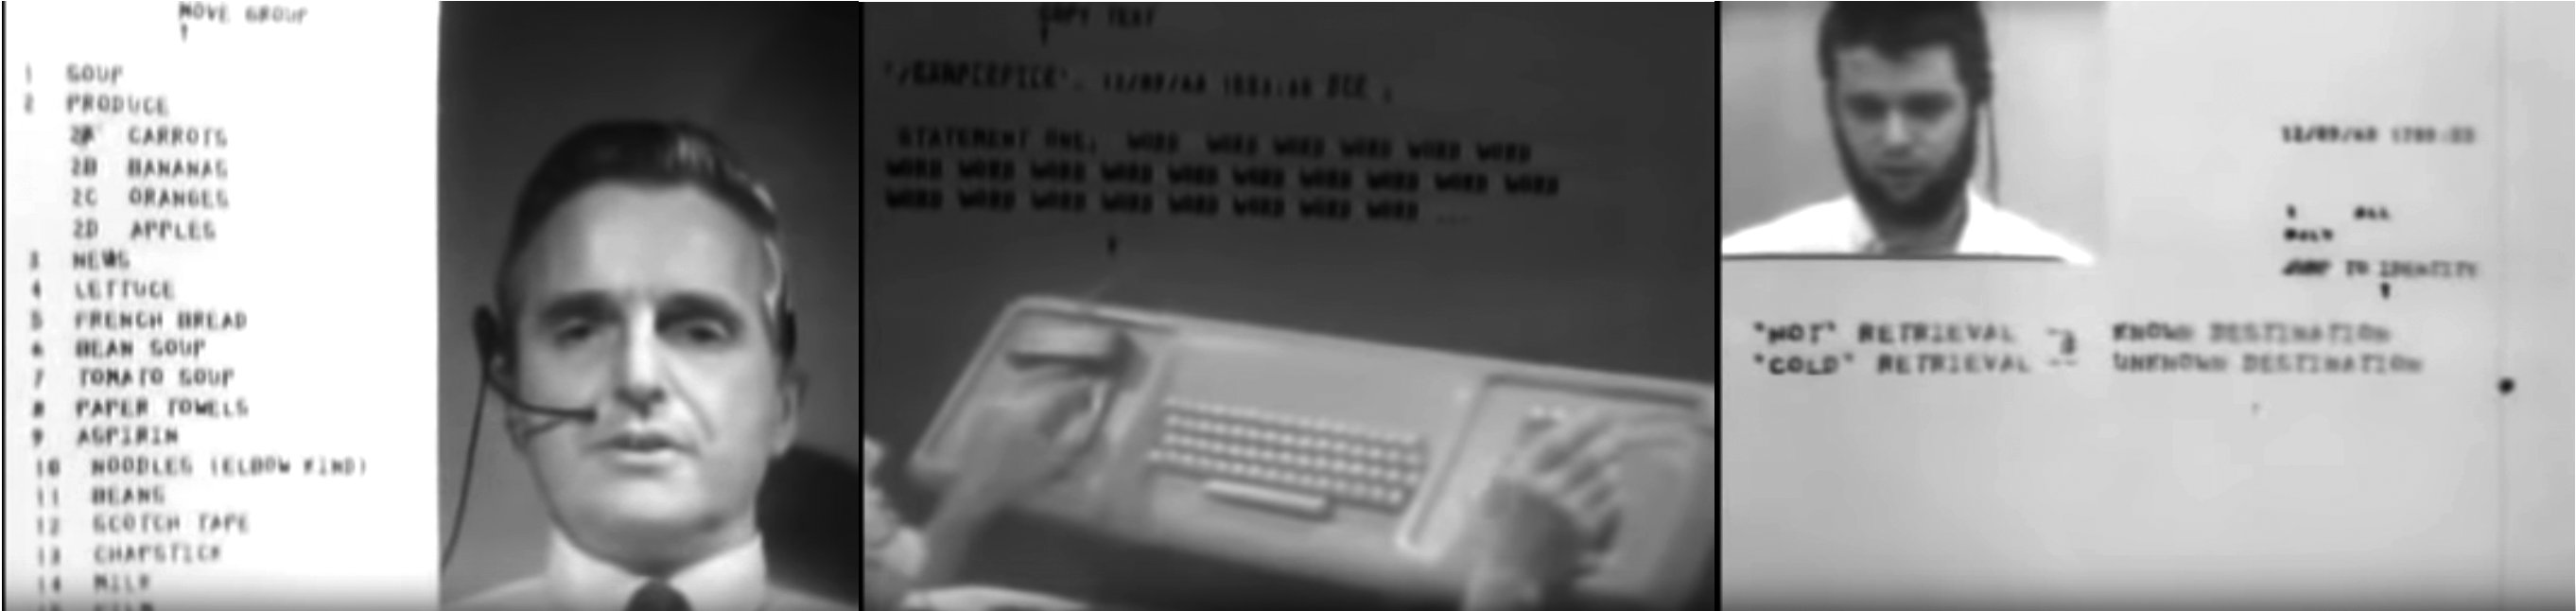
\includegraphics[width=1\linewidth]{pictures/cap2/mother_of_all}
    
    \legend{Fonte: Screenshot da autora do vídeo disponível em \url{https://youtu.be/yJDv-zdhzMY} no dia 20 de dez de 2017.}
\end{figure}



Pensar na ideia de \emph{bootstraping} como metodologia de trabalho fez, de uma certa maneira, mudar o foco inicial desta pesquisa, que era inicialmente de construir coisas genéricas para um usuário genérico --- como é tradicionalmente a metodologia do design --- para procurar construir instrumentos que fossem, acima de tudo, ferramentas para a nossa própria pesquisa prática em música experimental, individual e coletiva, junto a redes como NuSom, Sonora, Tecnoxamanismo, BlóKõKê, Orquestra Errante entre outras.

\subsubsection{\emph{Bootstrapping} na música}

Na história da música existe uma série de casos onde a ideia de desenvolver seus próprias tecnologias para produção sonora moveu parte da pesquisa dos músicos. Uma pessoa que teve essa abordagem foi Daphne Oram, precursora da música eletrônica que desenvolveu um sintetizador de música baseado em desenhos. O Oramics funcionava através de desenhos que definiam envelope, e perfil melódico do som. Oram observou que a música eletrônica dital na época era regida principalmente por ``processos impositivos'', principalmente baseados em tom, volume e duração, ou baseados em sons puros, como de osciladores, ou em desenhos de onda definidos digitalmente, que segundo ela ``tinham pouca finesse'' \footnote{\cite[p. 101]{Oram1972}}: 

\begin{citacao}
One of the points to notice in digital computer music is the
quality of each note ... its timbre, its subtlety, its individual shape and phrasing. When you come to program your digital computer will you, mostly, be concerned with the regulation of pitch and rhythm and interval relationship? Will you be able to give time, also, to considering the beauty of each individual note... the subtle individuality of each note ... as well as its place in the main scheme? Will each note, each phrase or melisma, be able to affirm the richness and the character of its own individuality, while it is taking its balanced position in the overall structure? 

We wish to design this machine-with-humanising-factors so that the composer can instruct it by means of a direct and simple language. He will want to transduce his thoughts as quickly as possible, via a channel which is logical. \footnote{\cite[p. 97]{Oram1972}}
\end{citacao}

Seu desejo era de criar uma máquina em que ela pudesse desenhar os sons, e para tanto, ela passou muitos anos desenvolvendo a ideia dessa máquina até que conseguiu recursos para construí-la. O Oramics, foi no entanto, uma máquina única, desenhada pela e para a própria autora --- na busca de expressar seus desejos estéticos composicionais --- e nunca chegou a ser um produto comercializado nem produzido em série.   

\begin{figure}
    \caption{\label{oram}Daphne Oram e o Oramics.}
    
        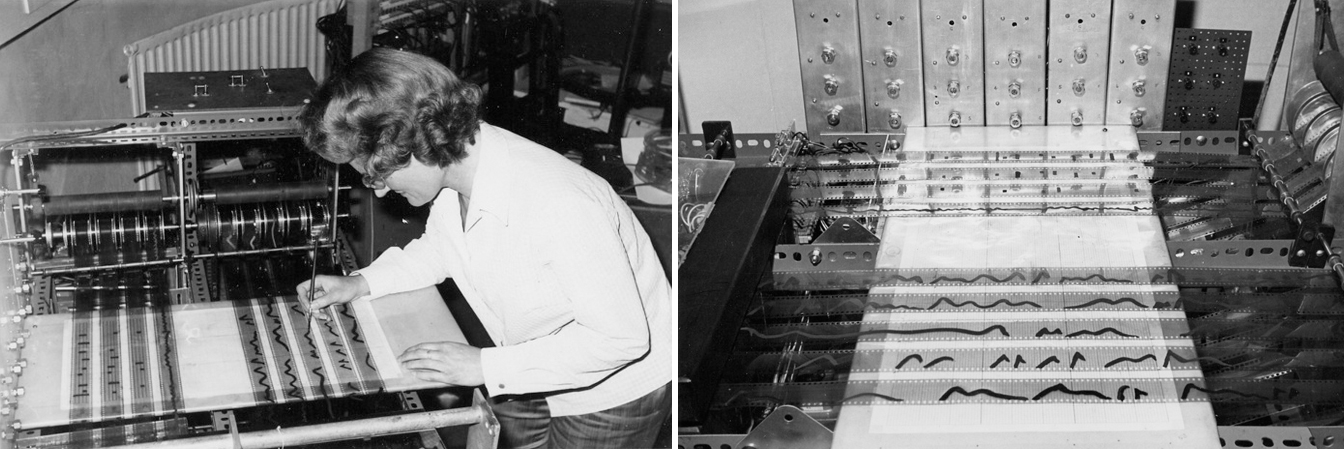
\includegraphics[width=1\linewidth]{pictures/cap2/oramics}
    
    \legend{Fonte: \cite{DavidCranmer2009}.}
\end{figure}


Outros que também desenvolveram seus próprios intrumentos para trabalhar com música foram os irmãos John and James Whitney, considerados precursores da música visual, que nos anos 60, criaram um sistema mecanizado baseado em um conjunto de pêndulos, capaz de escrever ondas senoidais na faixa de som de uma película cinematográfica; uma impressora sonora, como John explica abaixo:

\begin{citacao}
Nosso instrumento de som subsônico consistia em uma série de pêndulos ligados mecanicamente a uma cunha ótica. (...) Nenhum som audível era gerado pelo instrumento. Ao invés disso, uma trilha sonora ótica de dimensões padrão era sinteticamente exposta no filme, que depois de processado podia ser tocado em um projetor de filmes padrão."\footnote{\cite[p. 152]{Whitney1980}, tradução nossa} 
\end{citacao}

\begin{figure}
    \caption{\label{witney}Três imagem extraídas do filme ``Five Abstract Film Exercises'' de John e James Whitney.}
    
        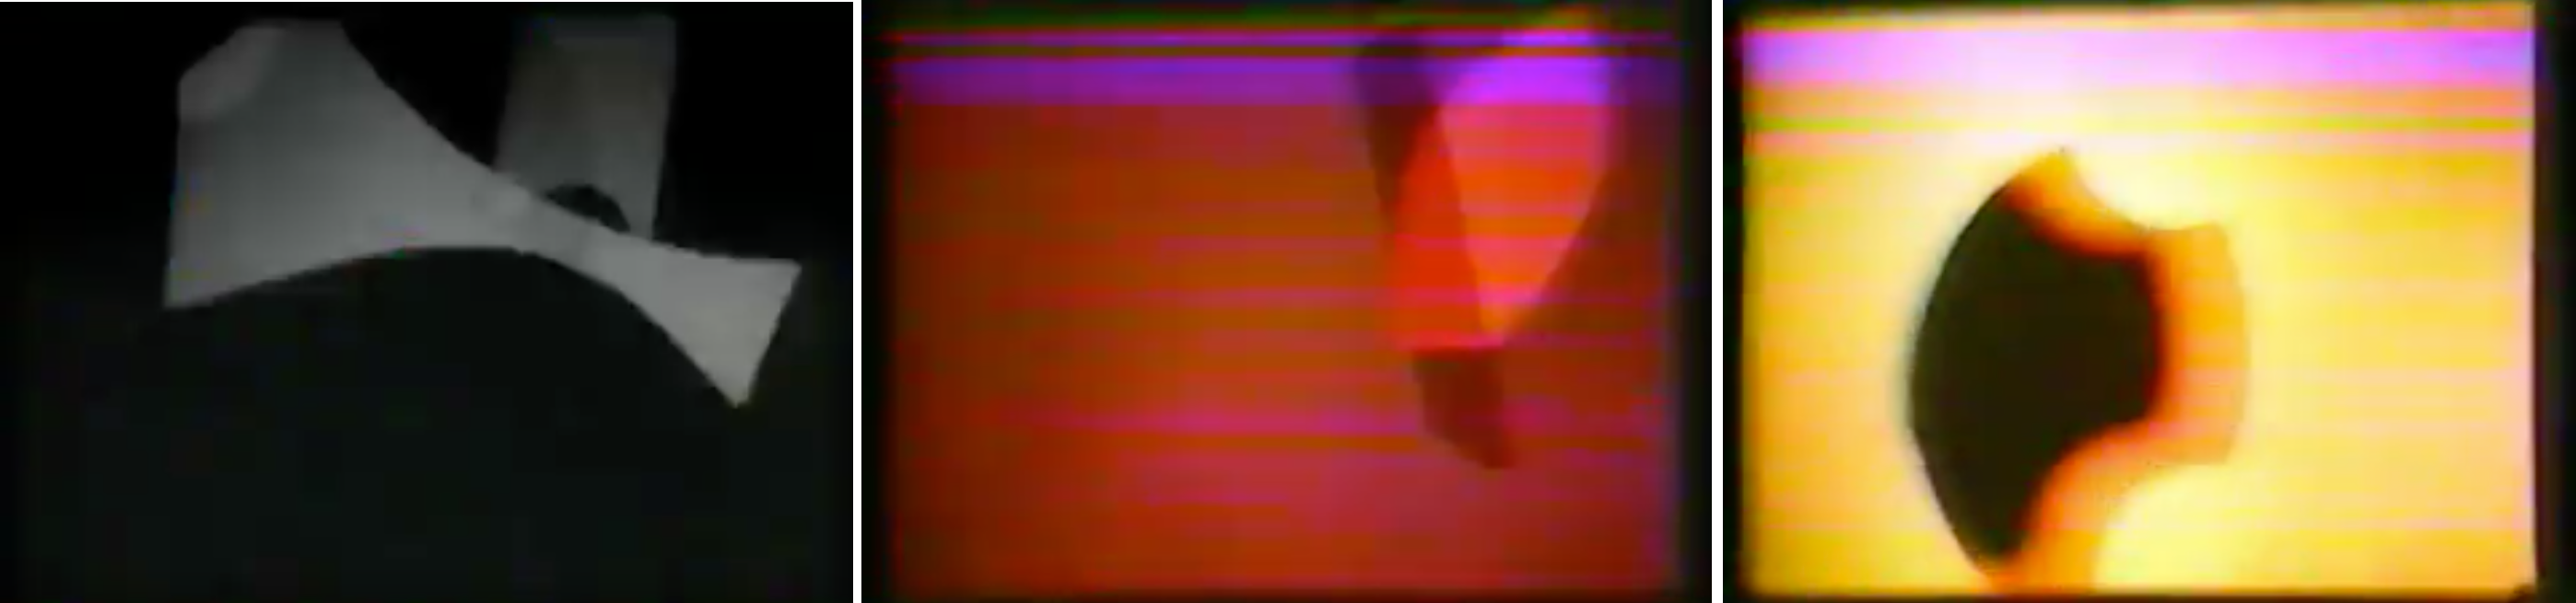
\includegraphics[width=1\linewidth]{pictures/cap2/witney}
    
    \legend{Fonte: Screenshots da autora.}
\end{figure}


Com esse instrumento, eles fizeram os filmes``Five Abstract Film Exercises''. O resultado sonoro, que trazia ondas puras senoidais e até glissandos foi chocante para época, e garantiu à dupla o prêmio pelo som na competição de filmes experimentais de Bruxelas de 1949\footnote{Disponível em: \url{https://www.youtube.com/watch?v=kuZbgM8yxtY}}.


Enquanto seu irmão James, foi com o tempo passando a se voltar mais à pintura e a questões místicas e de espiritualidade, John procurou a se dedicar mais ao desenvolvimento tecnológico e a sistematizar um pensamento sobre música e linguagem visual. Ao longo dos anos ele foi desenvolvendo um computador mecânico analógico, especialmente para animação com tipografia\footnote{\cite{Youngblood1970}}, prestando serviços para a indústria de filmes. Colaborou com Saul Bass na famosa abertura para o filme Vertigo, de Hitchcock, por exemplo. Sua máquina era formada por câmeras e mecanismos rotativos capazes de produzir imagens em movimento no filme a partir de moldes de cartolina e cálculos matemáticos complexos.  Whitney usou como base para seu primeiro computador analálogico um dispositivo antimísseis M-5, ressignificando um equipamento militar, ou nas palavras de Youngblood, ``uma arma da morte'' em uma máquina capaz de produzir beleza\footnote{\cite{Youngblood1970}}.

Suas pesquisas com o computador analógico levaram em 1966 a IBM se tornar a primeira empresa a abrigar um artista em residência, para explorar as potencialidades estéticas da computação. O filme ``Permutations'', seu primeiro desenvolvido em um computador digital, era considerado por John como o desenvolvimento de um novo modo de comunicação. Com a IBM, Whitney começou a trabalhar com o computador digital, que não exigia mais a necessidade dos estênceis analógicos. \footnote{\cite{Youngblood1970}}. 
Em seu livro ``Digital Harmony --- on the complementarity of musical and visual art'', publicado em 80, Whitney defende uma idéia de harmonia que ultrapassa a esfera da música, ``um contexto mais amplo no qual as leis Pitagóricas da harmonia operam''. Em seus filmes ``Permutations'' (1968) , ``Matrix I'' e ``III'' (1970 e 1972), e ``Arabesque'' (1973), Whitney programa formas em movimento segundo parâmetros matemáticos inspirados na harmonia de músicas de outros artistas, como Terry Rilley (Matrix III) por exemplo, procurando interpretar princípios harmônicos e rítmicos como formas e processos geométricos no tempo. Passou a perseguir a ideia da construção de um instrumento que fosse capaz de gerar som e imagem simultaneamente e em consonância. Esse instrumento partiria de parâmetros harmônicos do som, que eram mapeados em forma de coordenadas polares ou cartesianas. \footnote{\cite{Whitney1980}}

\begin{figure}
    \caption{\label{matrix}À esquerda, quadros do filme Matrix. À direita, a correlação gráfica da harmonia entre as notas musicais.
.}
    
        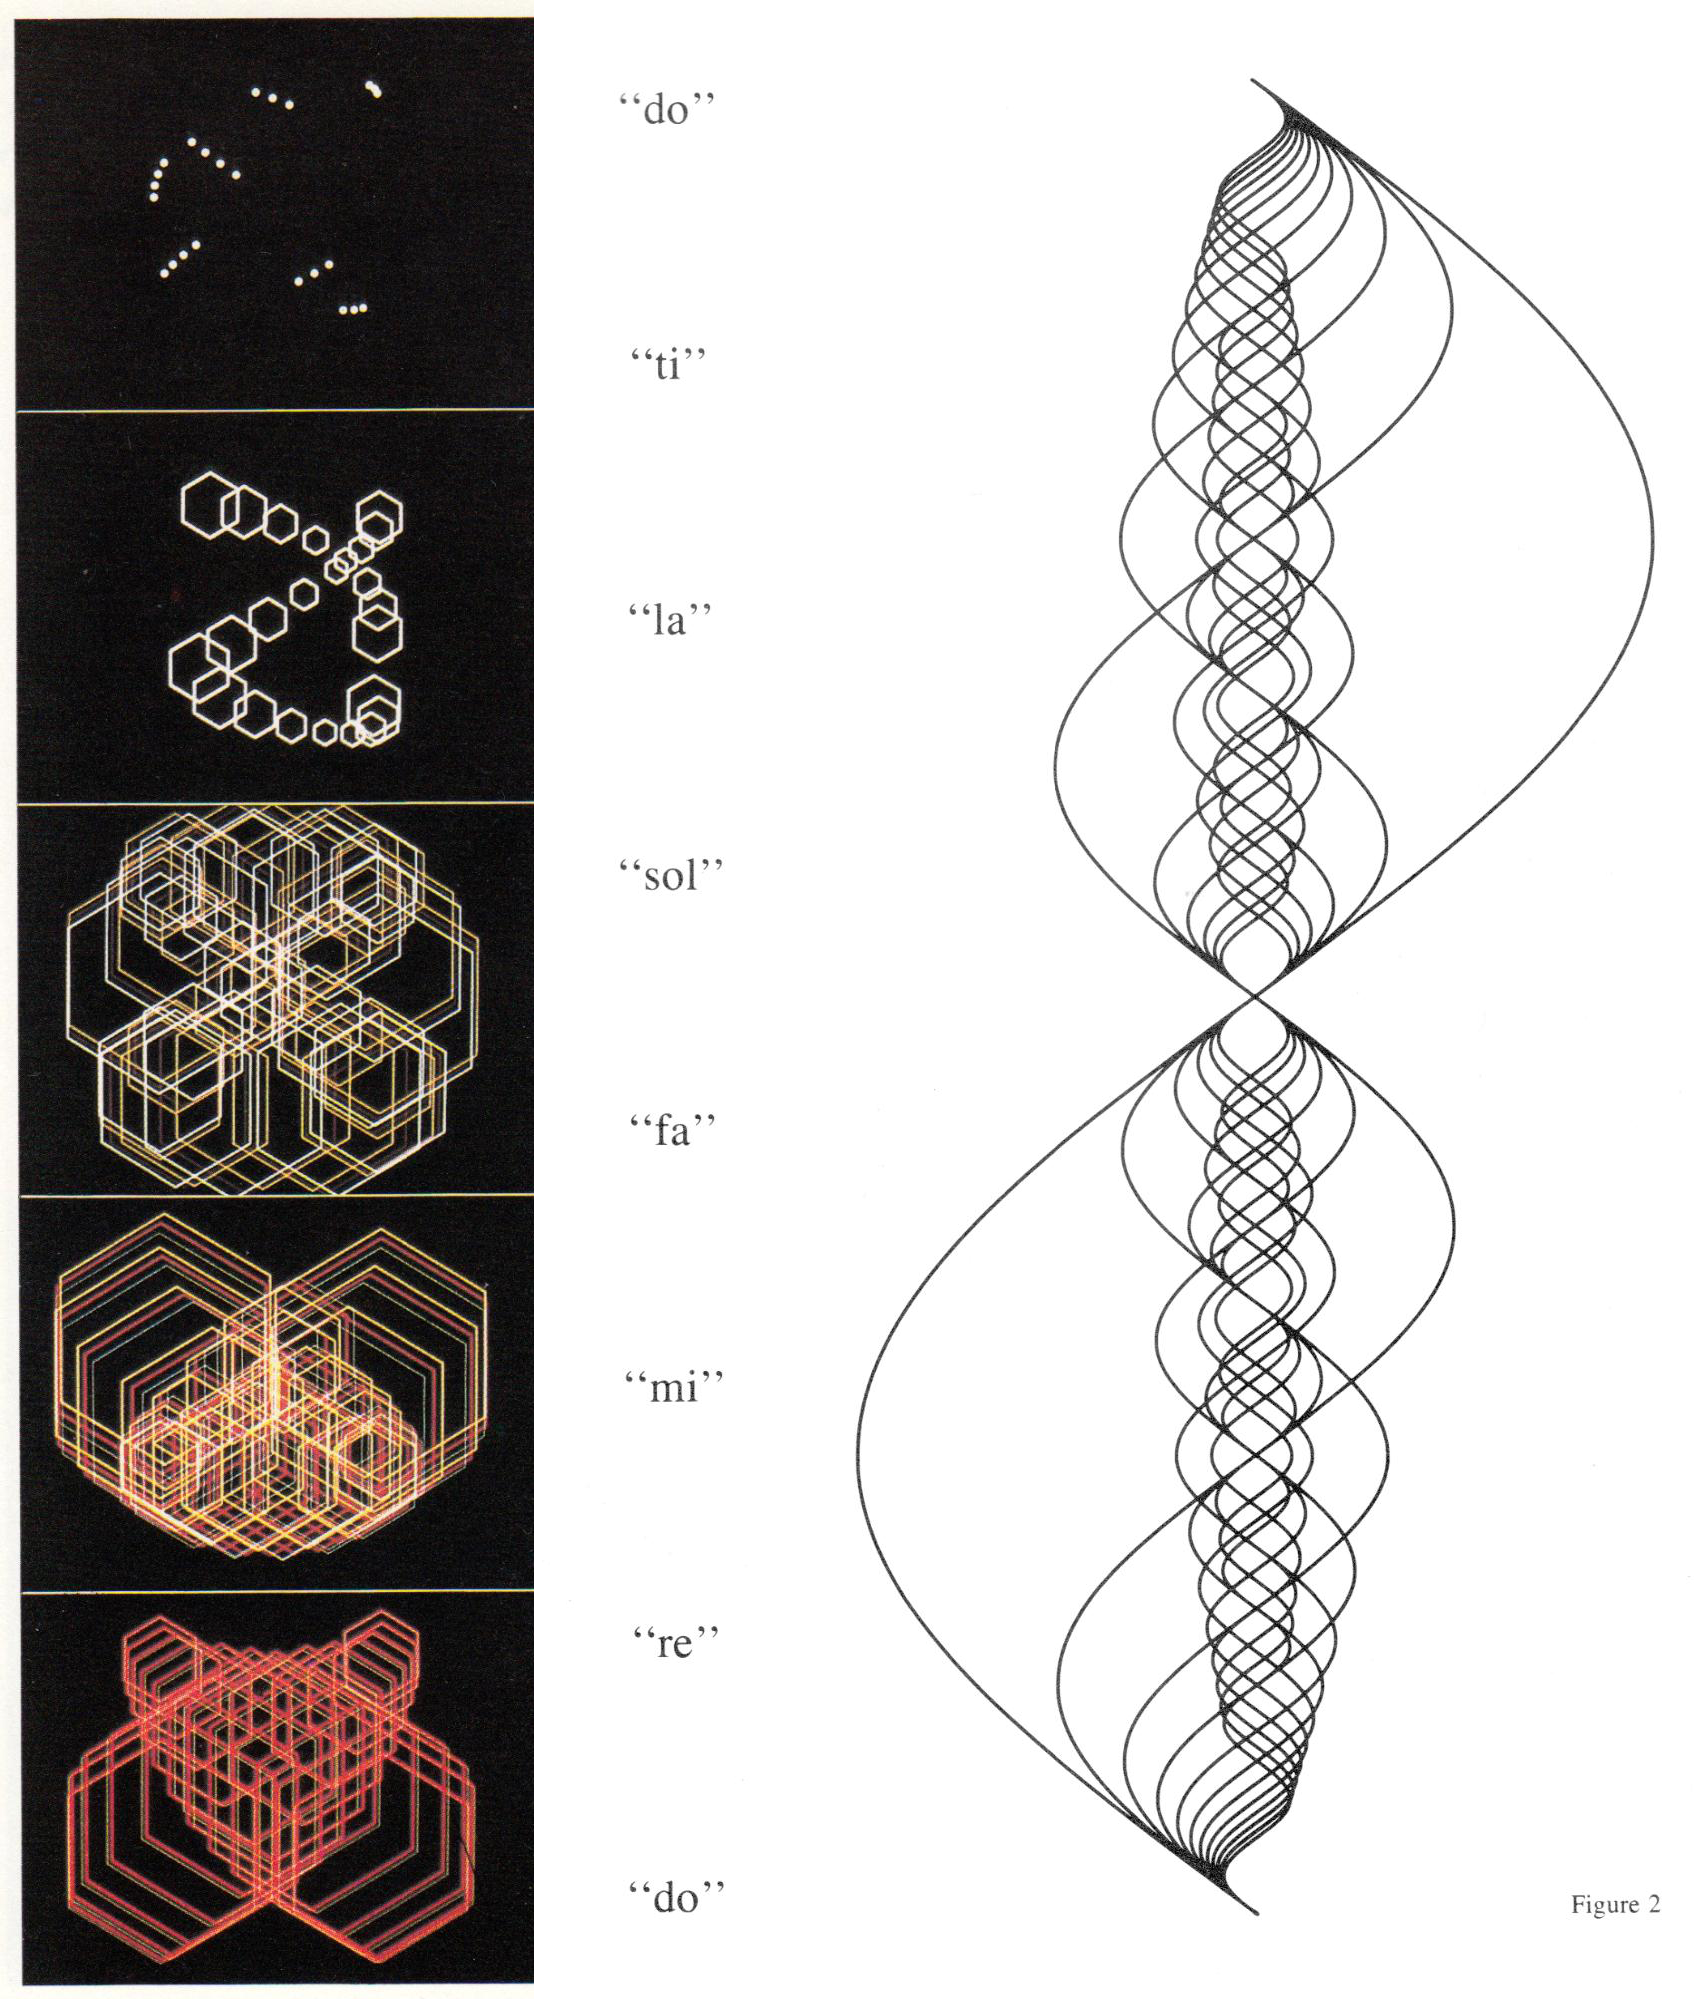
\includegraphics[width=0.8\linewidth]{pictures/cap2/witney2}
    
    \legend{Fonte: \cite{Whitney1980}}
\end{figure}


Outro que pesquisou com novas interfaces para produção de novas formas de música foi Iannis Xenakis, arquiteto e pioneiro na música experimental do século passado. Xenakis também foi vanguarda no pensamento da relação entre matemática, som e sua relação com arquitetura e o espaço, criando música a partir de relações matemáticas do desenho de frequências dentro do espectro sonoro. Desenvolveu novas formas de notação musical para abarcar suas experiências que fugiam do padrão tonal de composição tradicional, como aponta Crististiano Figueiró \citeyear{figueiro2013influencia}:

\begin{citacao}
Xenakis (1996), aponta o uso de um espaço multidimensional como auxiliar na representação das características de um som como um gráfico que auxilie a composição, ordenando cada característica de um som como altura, amplitude, tempo, densidade, desordem, parâmetros de timbre, etc..; onde cada característica é uma linha dimensional, e os sons, pontos paralelos em várias dimensões \cite{figueiro2013influencia}
\end{citacao}

Xenakis defendia que tudo é sujeito às leis da lógica e suas operações, como adição, subtração e intersecção, por exemplo, e sendo assim, "a música poderia ser definida como organização de operações elementares entre funções de entidades sonoras”.\footnote{\cite[p. 21]{Xenakis1971}}. Ele se amparou no desenvolvimento da tecnologia de processamento digital de áudio nos anos 70 para desenvolver, junto à sua equipe no ``Center for Studies in Mathematical and automated Music em Paris'' o UPIC, uma ferramenta capaz de converter desenhos em som, em uma correspondência direta entre posição horizontal das linhas na partitura e as frequências audíveis pelo ouvido humano.


\begin{figure}
    \caption{\label{xenakis}Trecho de \textit{Mycenae Alpha} de Iannis Xenakis.
.}
    
        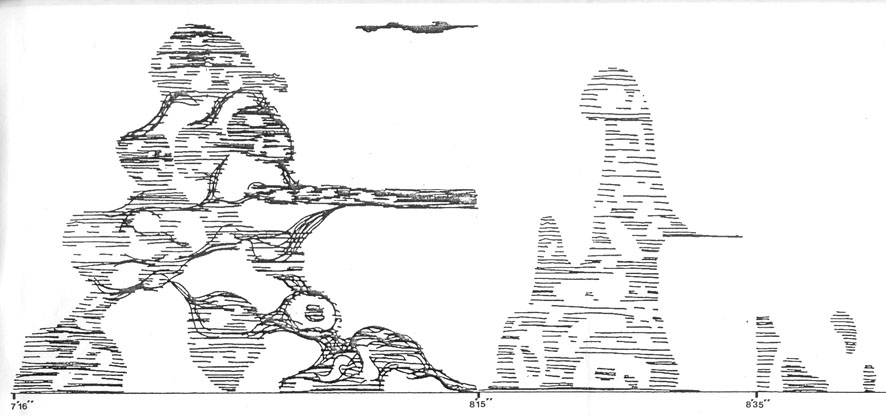
\includegraphics[width=1\linewidth]{pictures/cap2/metastasis}
    
    \legend{Fonte: \cite{Whitney1980}}
\end{figure}

%Uma outra referência importante para a pesquisa, está fora do campo do desenvolvimento de interfaces, a partitura visual de ``Artikulation'', de Gyorgy Ligeti, criada por Rainer Wehinger. Nela, as formas desenhadas correspodem a entidades sonoras da peça composta em fita. O trabalho não é uma representação literal do espectro gráfico da peça, mas uma leitura aproximada e sintetizada, num diálogo com princípios estéticos baseados também na teoria da forma (Gestalt).

%\begin{figure}
 %   \caption{\label{ligeti}Trecho da partitura visual criada por Rainer Wehinger para a peça Artikulation, de Giorgy Ligeti..}
    
 %       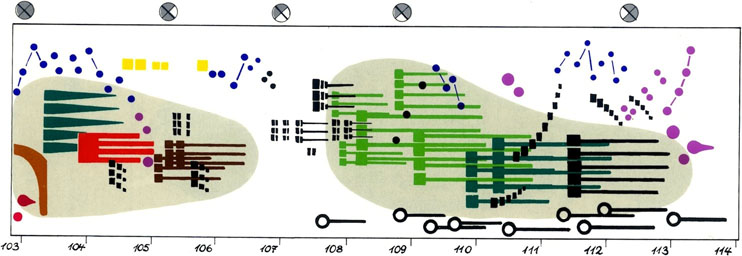
\includegraphics[width=1\linewidth]{pictures/cap2/ligeti}
    
  %  \legend{Fonte: \cite{Whitney1980}}
%\end{figure}


%\subsubsection{Brasil}
%Na cultura brasiliera, Anton Walter Smetak (Zurique, 1913 - Salvador, 1984), assim como o seu discípulo Marco Antônio Guimarães, são uma referência importante na pesquisa de intrumentos de invenção \footnote{\cite{Lima2018, Multimeios2001, Obici2014}}. Entre os princípios da sua prática estavam da pesquisa sonora de novos materiais, das necessidades do compositor ou do grupo, da modificação ou releitura de instrumentos tradicionais e da reciclagem de materiais diversos. Smetak construiu uma série de instrumentos que dividiu em algumas categorias: Instrumentos de sopro, percutidos, de percussão, a arco, plásticas sonoras, plásticas e instrumentos coletivos e diversos, que incluía um instrumento eletrônicos (o bicho) \footnote{\cite{Multimeios2001}}. 

%Seus instrumentos tinham uma forte característica escultórica, chegando a ``objetos plásticos de interatividade sonora'', como aponta Scarassati: ``de um lado o instrumento musical como um ponto de partida e, do outro, a escultura como um ponto de chegada, tendo a performance como a estrada que liga estes pólos''. Seus intrumentos, também não exigiam virtuosismo musical, como aponta o autor, facilitando seu uso no contexto de improvisação musical em grupo em que o compositor atuava. Também extraploavam os limites da música ocidental, abrindo perspectivas para o microtonalismo, onde segundo ele, ``não há o critério da afinação''. Smetak construiu cerca de 150 instrumentos musicais novos, ``utilizando materiais diversos, como cabaça, bambu, madeira, tubos de PVC, mangueiras plásticas etc.'' \footnote{\cite{Andres2011}}, movido por uma ``ideia de que uma nova humanidade requer uma nova música''. Em depoimento no vídeo documentário Smetak: Som e Espírito \citeyear{JessicaSmetakPaoli2010}, Smetak fala um pouco sobre sua inspiração:


%\begin{citacao}
%Cada objeto sonoro era um veículo para alcançar um novo plano de consciência. (...) Senti a responsabilidade que alguma coisa de mim devia se expandir, surgiram assim os primeiros intrumentos, qual batizei como nome de Choris, isso é, não chora nem ri. A improvisação um dia necessário para substituir a composição escrita. A idéia de um universo se aperfeiçoando, se ajustando com a interferência das artes e ciências em todos os setores. Efetuaram-se vários instrumentos de sons percutidos, os últimos com molas de aço amplificados eletrônicamente estourando-se na esfera da Caossonância que nos levou a múltiplas observações, mas levando sempre em consideração os citados dos sábios: ``que não há nada de novo embaixo do Sol''
%Tenho procurado diferenciar claramente o fazer som, um meio de despertar novas faculdades da percepção mental e o fazer música, apenas um acalento para velhas faculdades da consciência. \footnote{Walther Smetak, in \cite{JessicaSmetakPaoli2010}}
%\end{citacao}

%Quanto à autores contemporâneos, a tese de doutorado do pesquisador José Guilherme Allen de Lima \footnote{\cite{Lima2018}} ``Práticas de luteria na música experimental brasileira'', aprensenta uma panorama da luthieria experimental brasileira contemporânea, com uma pesquisa extensa de autores, espaços e tecnologias, principalmetne relativas a intrumentos físicos, muitos dos quais foram também desenvolvidos pelos próprios músicos que os tocam, como André Damião Bandeira, Cadós Snaches, Natacha Maurer e Marcelo Muniz, Arthur Jolly, Wilson Sukorsky, Pan\&Tone, LoopB entre outros.

%No campo da luthieria digital no Brasil, destacamos o trabalho de Jarbas Jacome, especialmente o ViMus, uma interface que faz a conversão em tempo real de áudio em imagens, e o trabalho de Jerônimo Barboza, que atualmente pesquisa na Universidade McGuill com Marcelo Wanderley, o Illusio, que parte de uma interface desenhável para criar um sistema de samplers capaz de gerar uma ``banda de um homem só''.  




%Thus, as discussed in (Fels, Gadd, \& Mulder, 2002), the task of keeping the adopter of the instrument engaged, involves designing for increasing complexity and expressivity as the player becomes expert.

%não se faz muita coisa sem software em música hoje em dia puckette

\subsubsection{Interfaces digitais}

Desde que os primeiros computadores estiveram disponíveis para pesquisa científica, músicos, compositores e pesquisadores têm desenvolvido interfaces para seu emprego em atividades musicais. Nos primeiros computadores a interface era física e a programação era operada por meio de cabos e potenciômetros diretamente no nível do hardware\footnote{\cite[p. 110]{Henrique1996}}. O ENIAC (1943 - 1946) (figura 1), um dos primeiros computadores construídos durante a Segunda Guerra Mundial com fins militares \footnote{\cite[p. 24]{Stolfi}}, era operado por pessoas com grau avançado de domínio da matemática, muitas das quais mulheres que já trabalhavam na guerra como computadoras fazendo manualmente cálculos de balística \footnote{\cite{HayleyWilliams2015}}, sua interface tem uma certa semelhança com a dos grandes sintetizadores modulares construídos anos depois, como o feito por Joseph Paradiso a partir de 1974, e que foi remontado em 2012 em uma exposição no MIT\ref{analogicos} de janeiro a abril de 2012. 

\begin{figure}
    \caption{\label{analogicos}À esquerda, interface do ENIAC.  À direita o sintetizador modular montado por Joseph Paradiso. }
    
    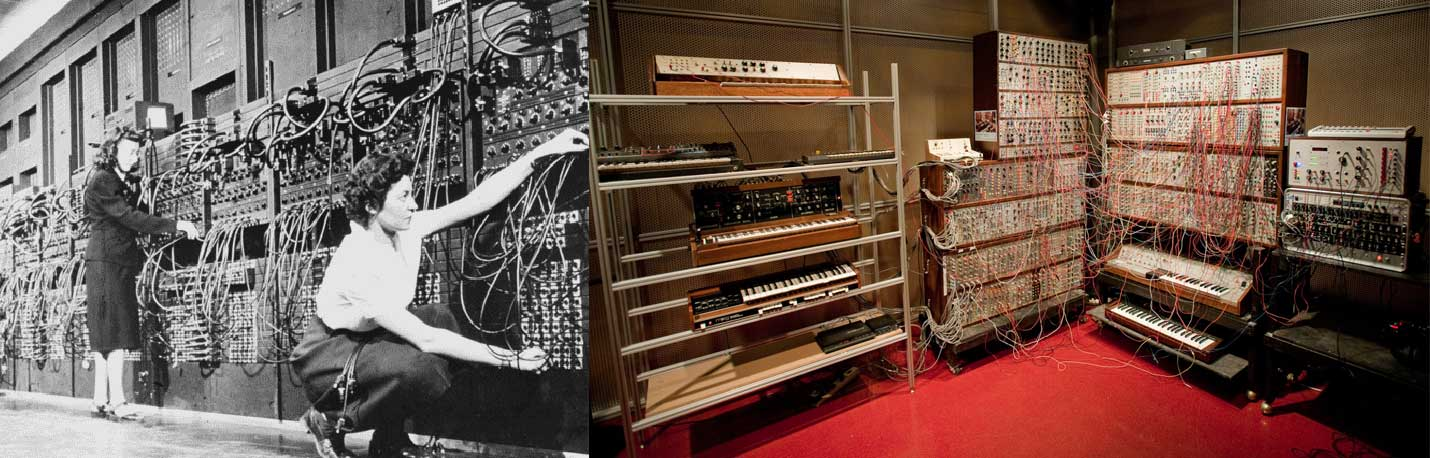
\includegraphics[width=1\linewidth]{pictures/analogicos}
    
    \legend{Fonte: \cite{HayleyWilliams2015} e http://web.media.mit.edu/~joep/pics/ FullSynthMIT-Museum.jpg}
\end{figure}

As primeiras experiências musicais em computadores digitais que se tem noticia foram realizadas na década de 50 por Max Mathews no ``Bell Telecom Lab''. Para gerar os primeiros sons computadorizados, Max teve que desenvolver uma linguagem de programação própria, que chamou de \emph{Music I} \footnote{\cite[p. 253]{Holmes1985}}. Depois de uma década desenvolvendo essa linguagem de programação musical, em 1968 passou a trabalhar no desenvolvimento do GROOVE (ou \emph{General Real-time Output Operations on Voltage-controlled Equipment}), um equipamento que funcionava na plataforma \emph{Graphic 1}, ``um sistema computadorizado interativo que podia traduzir imagens desenhadas com uma caneta luminosa em uma tela''\footnote{\cite[p. 253]{Holmes1985}}. Essa plataforma era similar à plataforma utilizada por Ivan Sutherland no \emph{Sketchpad}, pioneiro também dos programas de edição gráfica. O GROOVE teve a primeira interface gráfica interativa para computação musical. 

\begin{figure}
    \caption{\label{max}Max Mathews e L. Rosler com a estação de trabalho Graphic 1. }
    
        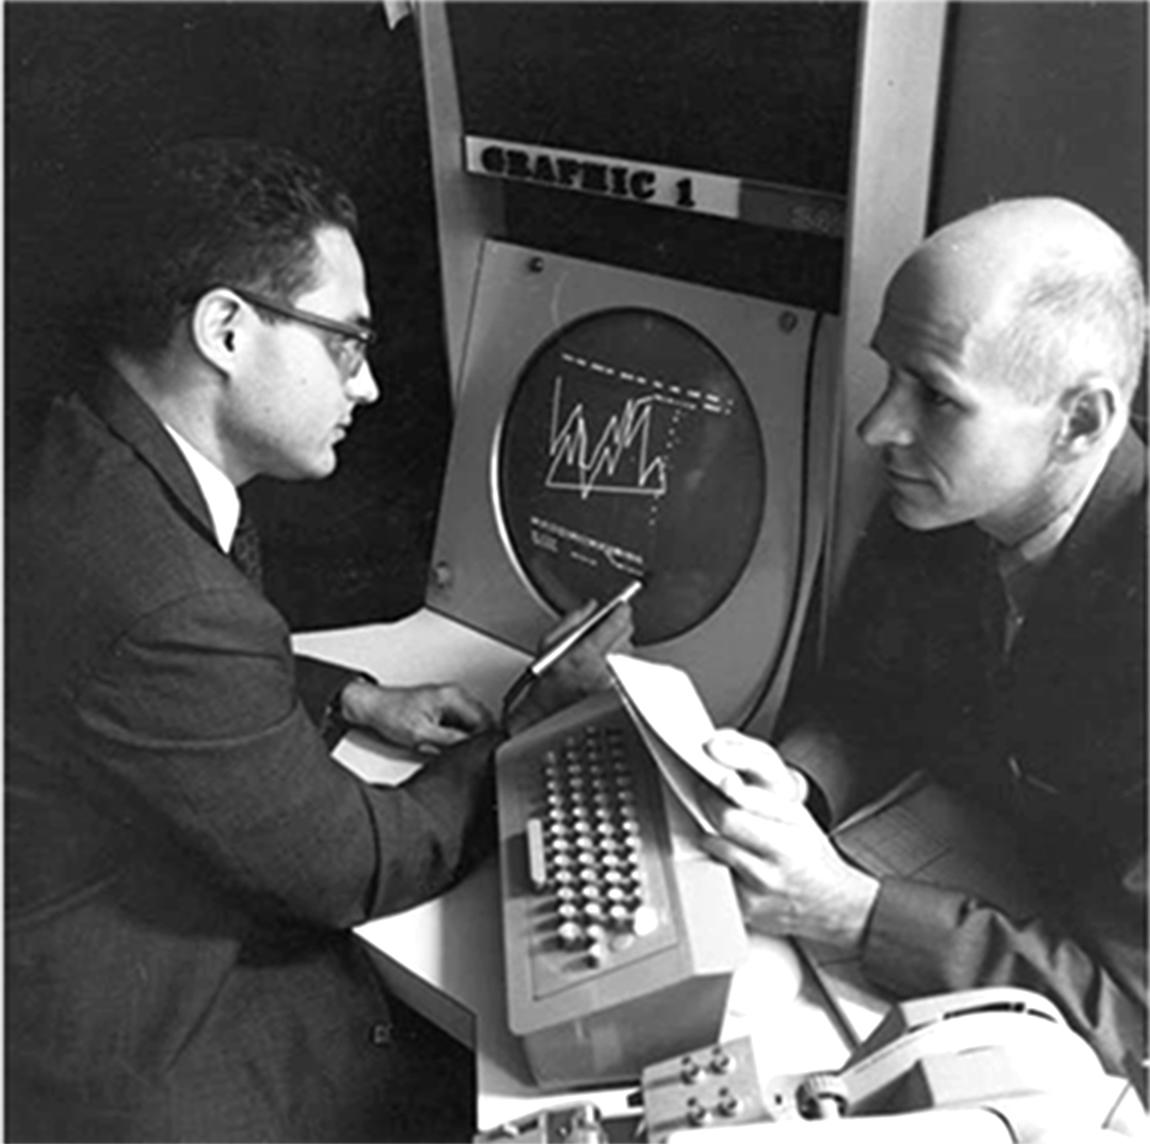
\includegraphics[width=0.5\linewidth]{pictures/MaxHolmes-251}
    
    \legend{Fonte: Holmes, 1985 p. 251}
\end{figure}

Com o desenvolvimento da computação surgiram também novas formas de interação e são desenvolvidas ``linguagens de programação mais eficiente e acessíveis'' \footnote{\cite[p. 111]{IAZZETTA1997}}. As próprias linguagens são interfaces que permitem a interação do programador com processos da máquina. Até o final da década de 70, compositores precisavam trabalhar diretamente com programadores para realizar qualquer tipo de trabalho em computação musical. Foi o caso de James Tenney, que trabalhou com Max Mathews no Bell Telecom Lab para a composição de 6 peças musicais ou o caso de Yannis Xenakis, que na década de 60 teve acesso aos laboratórios da IBM em Paris\footnote{\cite{Holmes1985}}, e empregou computadores na realização de cálculculos probabilísticos para a instrumentação de uma série de composições incluindo ``Atrées'' (1962), ``Morsima-Amorsima'' (1962) e as séries ``ST'' (ex. ST\/10\-1,080262 para dez instrumentos)\footnote{idem p. 263}.

Curtis Abbott, que escreveu o software da máquina 4C utilizada no final da década de 70 pelo IRCAM, começa seu artigo ``Music System Programming'' afirmando enfaticamente que ``programar é necessário para fazer qualquer coisa realmente nova em música computadorizada" \footnote{Abbot, C. in \cite[p. 51]{Roads1996}}. A computação musical é um das vertentes desse campo que desponta na produção artística moderna, que Abbot já definia nos anos 80 como ``programação criativa'', um campo da computação que vai lidar com questões artísticas e estéticas. 

Na metade da década de 70, foram lançados os primeiros sintetizadores digitais portáteis, o \emph{Synclavier}\footnote{\cite[p. 265]{Holmes1985}}, que tinha uma interafe similar ao do piano e custava entre \$200.000 e \$300.000 dólares\footnote{\cite{JosephParadiso1998}}, e posteriormente o \emph{Fairlight CMI}, que consistia em um sistema de processamento computadorizado, um monitor com caneta luminosa (lightpen), um teclado alfanumérico QWERTY, um teclado de 6 oitavas, além de um sistema de síntese analógica com 6 osciladores. Na época de seu lançamento o CMI original custava à partir de \$16.000 libras, o que não impediu que músicos famosos como Peter Gabriel, Kate Bush, Queen, Stevie Wonder, Herbie Hancock, Kraftwerk, Grace Jones, Frankie Goes To Hollywood, Thompson Twins, Human League, Tears for Fears entre outros o adotassem\footnote{\cite[p. 18]{Twyman2004}}. O CMI era uma ferramenta atrativa tanto para engenheiros da computação, pelo processador sofisticado, quanto para compositores, que podiam utilizá-lo para fazer orquestração complexa de suas peças, quanto para músicos, que podiam utilizá-lo em estúdio ou em performances ao vivo. Mas não era uma ferramenta tão simples de se operar como anunciava. \footnote{\cite[p. 55]{Twyman2004}}

Desde o lançamento do primeiro \emph{Macintosh}, que tinha uma interface gráfica mais amigável, uma gama de softwares para a produção musical floresceu, voltadas para profissionais de música, desenvolvimento de jogos e performers. Em 1990, uma parceria entre a \emph{Digidesign}, uma empresa que já desenvolvia softwares para produção musical e a \emph{Opcode}, que era a maior fabricante de interfaces MIDI na década de 80 gerou o Studio Vision, que podia ser comprado por \$950 dólares e foi o primeiro a integrar gravação e edição de áudio e MIDI, sendo considerado o primeiro software do tipo digital audio workstation (DAW). Sua interface gráfica misturava conceitos desenvolvidos nos primeiros editores de áudio, como a representação do som através dos gráficos de amplitude por tempo, com um piano-roll, para marcação de notas em função do tempo. Isso ajudou a aproximar músicos que usavam editores de partitura digitais \footnote{\cite{ChrisHalaby2011}}. A interface de edição multipista permite gravar várias faixas e sobrepô-las paralelamente no espaço gráfico da tela, o que dá ao produtor musical a possibilidade de organização visual do fluxo sonoro ao longo do tempo, permitindo ajustes mais precisos de sincronização e mixagem. A Digidesign, que posteriormente veio se tornar a AVID, foi se desenvolvendo continuamente até dominar o mercado de gravação digital com as várias versões do Pro Tools que foram lançadas desde 1991 com sistemas integrados de hardware e software voltados para estúdios. Graças a uma placa de áudio que podia ser acoplada externamente ao Mac, o sistema de áudio permitia gravação multipista, processamento de sinal e sistema de mixagem sofisticados, que eram mais baratos que os sistemas de hardware disponíveis na época. \footnote{\cite{ChrisHalaby2011}}.

Para facilitar uma aproximação com os profissionais que já trabalhavam nos estúdios analógicos tradicionais, o sistema contava com uma interface gráfica de usuário que se apoiava na mimese do estúdio tradicional de gravação em fita. Assim, elementos familiares dos técnicos de estúdio foram copiados de uma maneira literal, sliders, displays luminosos, potenciômetros rotativos, botões de controle como play, pause e stop e somados ao modelo de interface de edição multipista desenvolvida no Studio Vision. 

A cada versão do software lançada há um pequeno redesenho da interface gráfica, no sentido de acomodar mais recursos que são incluídos, mas também no sentido de tornar a interface mais “realista”, ou mais similar como imitação do estúdio de gravação analógica, com a inclusão de sombras, reflexos e degradês. Esses detalhes na prática não acrescentam nenhuma funcionalidade extra ao programa, na prática é possível que até prejudiquem, na medida que exigem gráficos mais pesados em termo de resolução e processamento gráfico, e nesse sentido servem somente para alimentar uma ideia de materialidade, dando ao software uma característica fantasiosa de objeto físico. 

Ferramentas como o Pro Tools, se enquadram no modelo que é chamado de \emph{Digital Audio Workstation} (DAW). DAWs são ferramentas que procuram emular de alguma maneira ferramentas do estúdio tradicional de fita, e como discuti no artigo ``Graphic Interfaces for Computer Music'' \footnote{\cite{Stolfi2016}}, tendem também a ter uma interface que busca mimetizar o equipamento de estúdio, em especial os controles giratórios e sliders, que são de difícil manipulação com mouse e teclados. Músicos profissionais no entanto, dispõe ainda muitas vezes de uma série de equipamentos auxiliares para isso, como controladores MIDI, mesas de som automatizadas e interfaces de áudio. O Pro Tools, por exemplo que foi por muitos anos um dos principais softwares de apoio aos estúdios tradicionais, era propagandeado como um sistema que integrado de hardware e software para produção musical. Sua interface imitava a tradicional mesa de mixagem de uma maneira quase literal, incorporando o desenho de amplitude de onda como forma de visualização padrão para os arquivos digitais como podemos ver na Figura \ref{protools}, retirada do site da empresa no início desta pesquisa.


\begin{figure}
    \caption{\label{protools}Interface do Pro Tools em 2015 }
    
        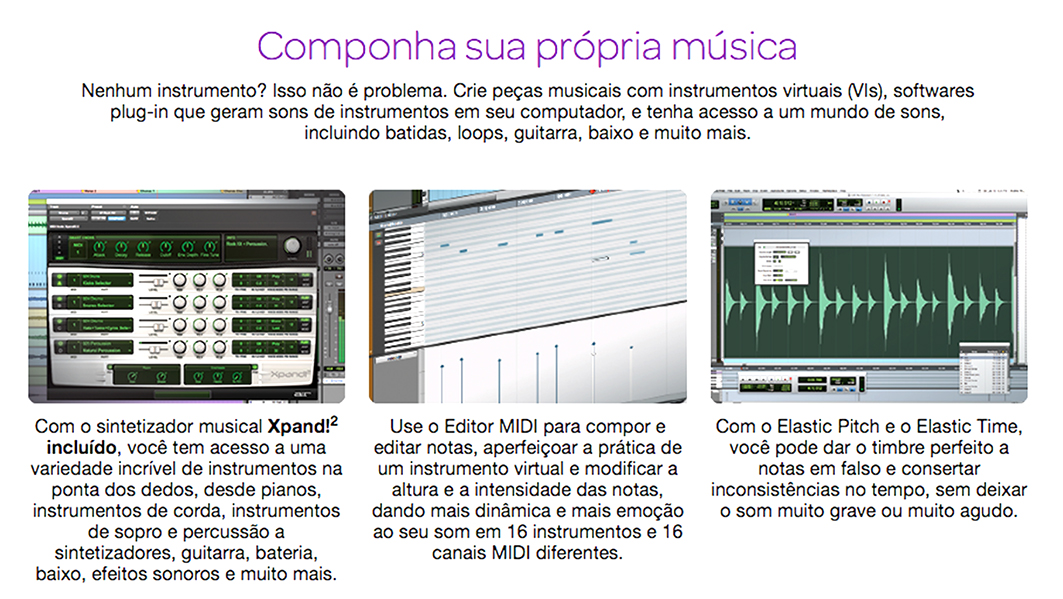
\includegraphics[width=0.8\linewidth]{pictures/protools}
        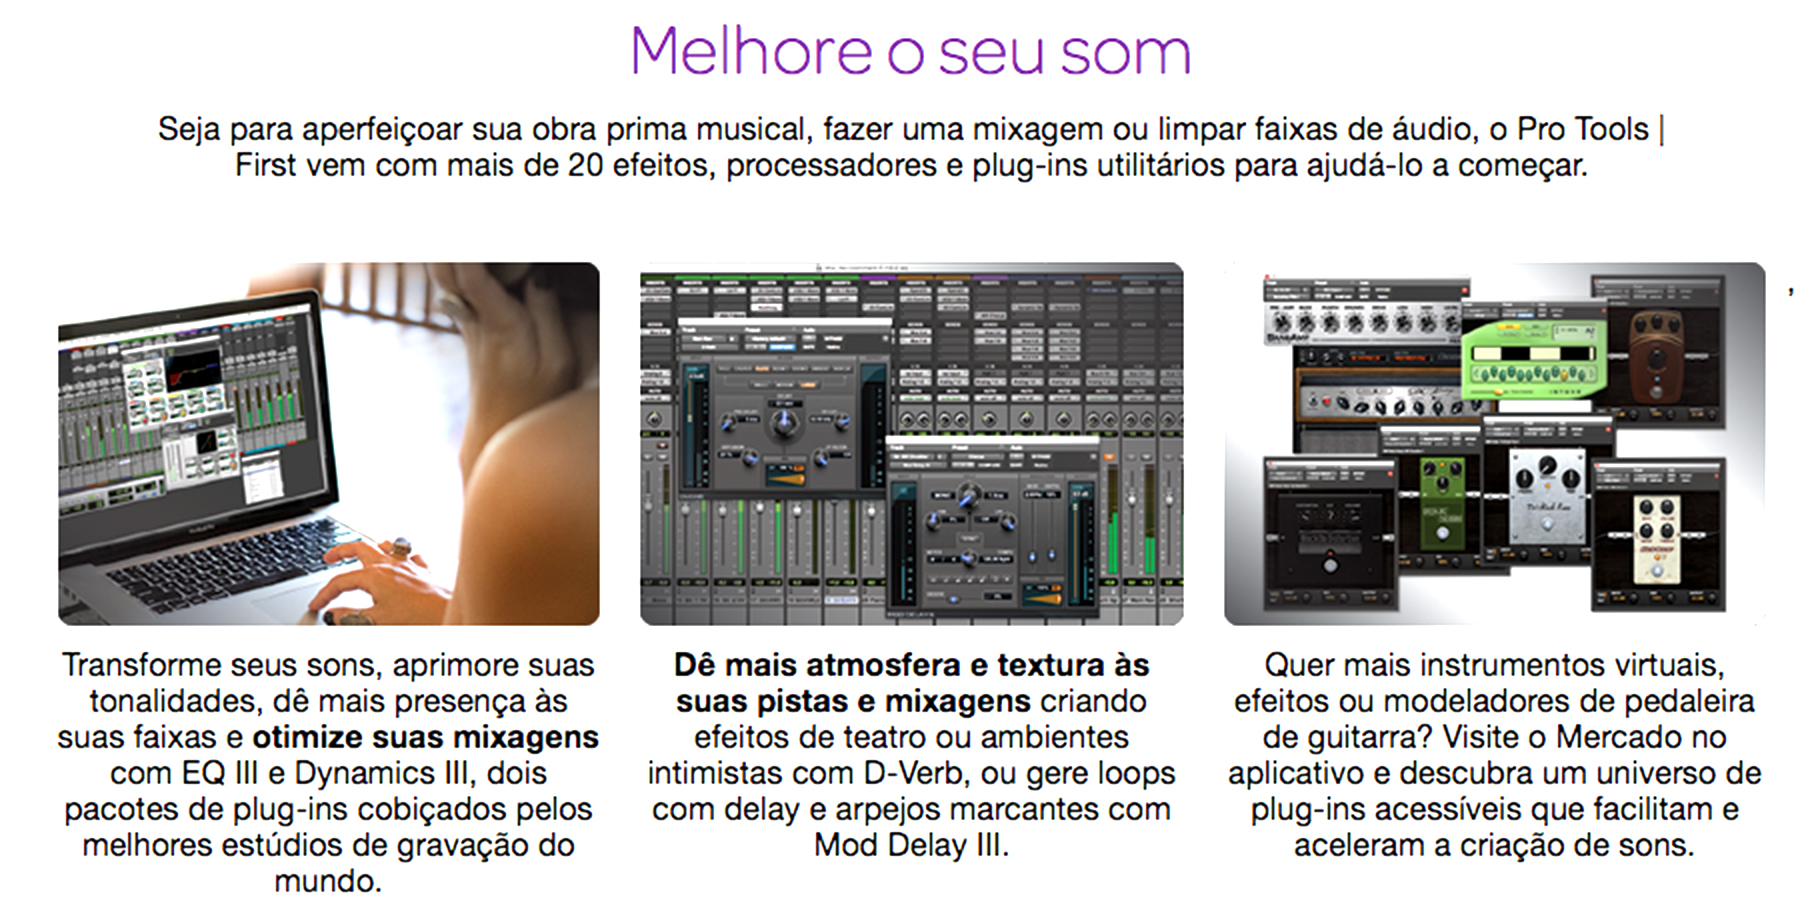
\includegraphics[width=0.8\linewidth]{pictures/protools2}
    
    \legend{Fonte: Print Screen da Autora em 17 de dezembro de 2015. Site: https://www.avid.com/pro-tools-first}
\end{figure}

Outro paradigma de software voltado para produção musical é o dos programas que permitem ao usuário o design de seus próprios aplicativos, como o Pd e o Max. Em 1986, Miller Puckette estava no IRCAM desenvolvendo um software chamado Patcher (um sistema gráfico para produção musical em tempo real para controlar a configurações de objetos no sistema MAX – um ambiente de programação orientada a objetos baseado em janelas voltado para produção musical, que na época rodava em um Macintosh, mas que já rodava no Synclavier II). O Patcher criava um sistema gráfico que simulava o sistema de cabos dos sintetizadores analógicos (figura \ref{analogicos}) e mecanismos de abstração que permitiam condensar módulos criando entradas e saídas que poderiam ser conectadas entre si. Tratava-se na visão de Puckette, um sistema que permitiria que ``os músicos escolhessem dentro de uma ampla gama de possibilidade, desenhando diagramas de fluxo de mensagem" \footnote{\cite[p. 5]{PucketteMiller}}. 

\begin{figure}
    \caption{\label{patcher}À esquerda, um exemplo de patch feito no software Patcher de 1988, e à direita, objetos pré-programados e elementos de controle para configuração da interface gráfica.}
    
        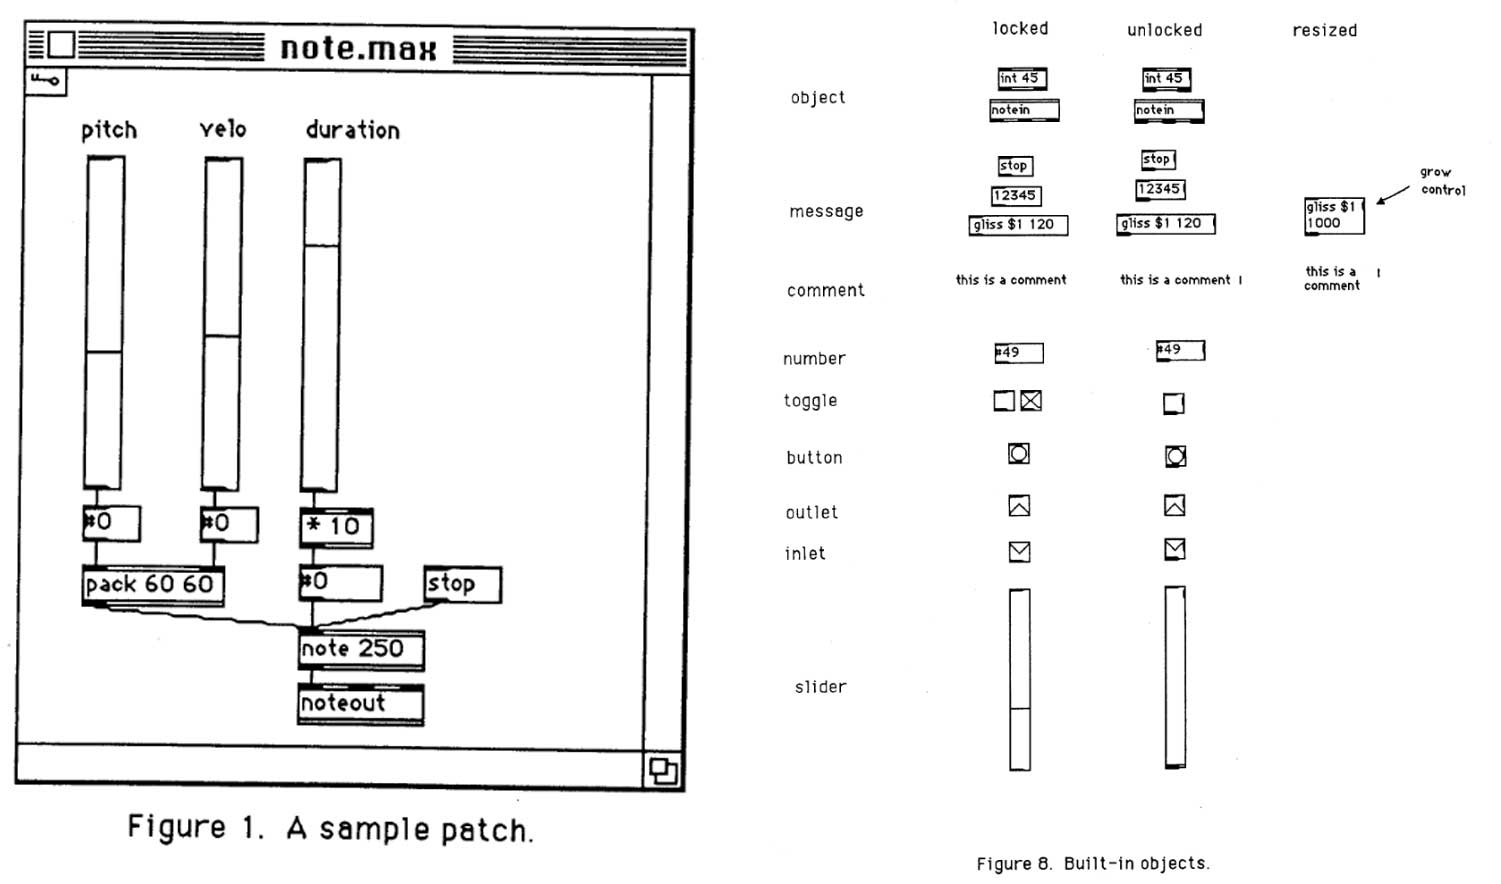
\includegraphics[width=1\linewidth]{pictures/cap2/patcher}
    
    \legend{Fonte: \cite[p. 6,9]{PucketteMiller}}
\end{figure}


Em 1990 o Patcher foi licenciado à Opcode e foi comercializado como Max\/Opcode, passando a ser desenvolvido por David Zicarelli. Em meados dos anos 90 a produção do software foi descontinuada pela Opcode, enquanto Miller Puckette continuou o desenvolvimento do programa no IRCAM que levou ao Max\/FTS (Faster than sound). Em 1996, Miller redesenhou totalmente o software e o lançou como um programa gratuito de código aberto chamado Pure Data (Pd), com uma interface gráfica muito semelhante à do Patcher original e das primeiras versões do Max. No ano seguinte, Zicarelli fundou a Cycling 74, que continuou o desenvolvimento e comercialização do Max\/MSP (abreviação tanto de Max Signal Processing ou de Miller S. Puckette) até os dias de hoje como software proprietário \footnote{\cite{Cryer2018}}.


\emph{Patchers}, como o Pd e o Max, podem permitir a construção de interfaces complexas e adaptadas para necessidades específicas de músicos e artistas, mas possuem uma linguagem mais complexa e exigem um conhecimento especializado de quem as programa. O Pd é, de uma certa forma, uma metáfora de ``bancada para o design de instrumentos musicais eletrônicos para performance musical ao vivo", com objetos pré programados que podem ser conectados para que os artistas criem seus próprios instrumentos de acordo com necessidades específicas. \footnote{\cite{PucketteMiller}}
 
Por mais que programas como \emph{patchers} sejam tentativas de prover o músico com um leque ampliado de potencialidaes criativas, as ferramentas  são em geral também formas de restrição das potencialidades musicais, como aponta Puckette (\citeyear{PucketteMiller}):

\begin{citacao}
 O desenvolvedor de software se esforça para impor o mínimo de restrições estilísticas possíveis sobre o musicista. No entanto, toda nova geração de software que surge revela possibilidades que, de alguma forma, não foram possíveis, ou pelo menos não encorajadas, pela geração anterior. Logo iremos aprender que, não importa o quão generosos ou poderosos sejam os softwares atuais, eles estavam de fato impregnados de suposições tácitas sobre como fazer música que restringem o campo das possibilidades musicais.

%Musicians can’t do much today without software, and so they are dependent on software developers. Software developers in turn are dependent on “users” (the musicians) to make artistic creations with their software; without that, the work of software development is pointless. The software developer strives to impose as few stylistic restrictions as possible on the musician. Yet every new generation of software that comes along reveals possibilities that were somehow not made possible, or at least not encouraged, by the previous generation. Soon we will learn that, no matter how general and powerful we believe today’s software to be, it was in fact steeped in tacit assumptions about music making that restrict the field of musical possibility. \footnote{\cite{PucketteMiller}}
\end{citacao}

%Complexity is not the same thing as expressive power. One wants one’s software to have the greatest expressive power possible, in the simplest possible way. \cite{PucketteMiller}

%\begin{citacao}
%There is also a more subtle, and perhaps more fundamental, aim: to make it so that the software doesn’t impose one or another stylistic bias on the musician. Such a bias might be easy to spot (a built-in set of available time signatures or musical scales, for instance), or might be so ingrained as to be almost invisible (for example, Max’s and Pd’s orientation toward reactivity that seems to privilege some approaches to real-time performance over others).
%\end{citacao}

\subsubsection{New Interfaces for Music Expression}


%\todo[inline]{outras práticas da comunidade NIME} 

Existe no meio acadêmico um volume expressivo de trabalhos e artigos que tratam das capacidades e de aspectos mais técnicos da computação musical, como o livro de Dan Hosken, ``Introduction to Music Technology'' (2011) e as publicações de Curtis Roads Computer ``Music Tutorial'' (1996) e Foundations do Computer Music (1985), ou sobre história da computação musical, como o trabalho de Thom Holmes, ``Electronic and Experimental Music: Technology, Music, and Culture'', (1985), mas provavelmente, o maior volume de pesquisa no campo da interface para produção musical é no desenvolvimento do que chamamos de ``NIME''. 

Em 2001, um grupo de pesquisadores propôs para a conferência CHI (Conference on Human Factors in Computing Systems), uma das mais importantes conferências em estudos do campo de interação humano computador (IHC) um workshop sobre ``New Interfaces for Music Expression'', embasados no rápido desenvolvimento das novas tecnologias digitais e eletrônicas, que estavam trazendo novas potencialidades para o campo de pesquisa de tecnologia musical. Entre seus objetivos estavam pesquisar e discutir o estado atual de ferramentas de controle para performance musical; identificar questões relacionadas entre mudanças de tecnologias e mudanças nas formas musicais; identificar como controles alternativos afetavam a expressão musical e o processo criativo de uma maneira geral e reunir experiências de trabalhos e estratégias dos participantes para resolver questões da área\footnote{\cite{Poupyrev2001}}. Depois deste primeiro \emph{workshop}, NIME se tornou uma conferência própria, que acontece anualmente reunindo diversos trabalhos de pesquisa e desenvolvimento de interfaces experimentais --- físicas ou digitais. 


Overholt (2009), quando define o ``espaço do design das tecnologias de interfaces musicais'', foca na questão do mapeamento e categorização dos gestos, que é uma posição mais ligada à ergonomia. O pesquisador Marcelo Wanderley, da universidade McGill, é um dos que vêm pesquisando a questão do mapeamento do gesto musical em novas interfaces para computação musical, no livro ``New Digital Instruments: control and interaction Beyond the keyborad'', escrito em conjunto com Eduardo Reck Miranda, eles tratam de diversas abordagens desenvolvidas nos últimos anos nesse sentido, como captura de gestos através de câmeras ou dispositivos baseados em sensores e software\footnote{\cite[p. 67]{Miranda2006}}. 

%cultura digital potencializou pesquisa em NIME

O compositor Eduardo Reck Miranda, que também é um dos cientistas brasileiros com produção mais significativa no NIME, desenvolve pesquisa de ponta na área de tecnologia musical, com estudos que incluem o uso de inteligência artificial para composição musical, por exemplo, no trabalho ``Caossynth'' \citeyear{Miranda2016}, e também têm explorado o uso de ciência biomolecular em composições mais recentes como ``DNA: Artibiotics'' \citeyear{miranda2018artibiotics}, que utiliza moléculas de DNA sintetizadas como agentes para composição musical.


Muito do trabalho desenvolvido no campo dessas novas interfaces, no entanto, é direcionado a um músico virtuoso, com grande domínio de técnicas musicais, como aponta Yina Blaine, uma das propositoras do primeiro workshop NIME de 2001:

\begin{citacao}
Talvez como um reflexo da visão Ocidental dominante de que música deva ser tocada apenas por músicos, a maioria dos trabalhos utilizando novas interfaces para expressão musical dos últimos trinta anos é orientada principalmente para experiências e performances virtuosísticas. Com intrumentos em estilo virtuoso, o designer pode rasoalvelmente esperar que o musicista vá investir uma quantidade tempo significativa em aprender as idiossincrasias do instrumento.
%Perhaps as a reflection of the dominant Western view that music should be played only by musicians, most work in the last thirty years using new interfaces for musical expression is primarily oriented toward virtuosic experiences and performances. With virtuoso-style instruments, the designer can reasonably expect the player to invest a significant amount of time learning the idiosyncrasies of the instrument. \cite{Blaine2003}
\end{citacao}



\subsubsection{Experiências em Web Audio}
Enquanto as produções em NIME costumam ser dedicadas à musicos virtuosos ou com grande nível de conhecimento técnico, exite também um campo de pesquisa em música ubíqua (UBIMUS)\footnote{\cite{Keller}}, que procura desenvolver ferramentas para o suporte criativo de atividades musicais para um grupo maior de pessoas, devido às possibilidades ampliadas de acesso oferecidas pelas tecnologias de rede e dispositivos móveis, ou nas palavras de Pimenta, Keller e Lazarini (\citeyear{Keller}):

\begin{citacao}
Um dos nossos objetivos é o de desenvolver ferramentas que tirem vantage desse contexto inclusivo, provendo condições para que noviços interessados em música participem de atividades criativas, em qualquer lugar e em qualquer momento, usando os dispositivos convencionais de comunicação móvel ou de computação que eles já possuam, e sejam familiares. \cite[p. 13]{Keller}

\end{citacao}

%One of our goals is to develop tools which take advantage of these inclusive contexts, providing conditions to novices interested in music to participate in creative activities, in any place and at any moment, using the very conventional mobile communications and computing devices that they already own, and are familiar

Quando inciamos essa pesquisa, já haviam alguns produtos de programação criativa disponíveis que estavam explorando esses novos recursos de Web Audio como suporte. Como forma de sistematizar a pesquisa, fizemos um levantamento de experimentos organizados pelo site ``Chrome Experiments'' que reúne milhares de casos de uso produzidos pela comunidade de ``programação criativa''\footnote{Disponível na url: \url{https://experiments.withgoogle.com/experiments}}. Em julho de 2016, apenas na categoria ``Sound and Music''  haviam listados 138 experimentos, desses uma série deles são experimentos estéticos com música generativa, jogos sonoros, videoclipes interativos, visualizadores de áudio, mixers e tocadores de MIDI, e alguns podiam ser considerados instrumentos musicais. Entre eles encontramos vários exemplos de sintetizadores, \emph{samplers}, processadores de áudio e sequenciadores, mas a maioria deles tinha como interface algo que mimetizam algum instrumento analógico ou eletrônico, principalmente o piano.

Encontrei algumas possibilidades interessantes como as experiências ``Lalo.li'' \footnote{Disponível em: <http://lalo.li/> }, que faz síntese de voz a partir de texto digitado na tela, podendo o usuário mudar o tom e a velocidade da voz. Sua interface é pareceida com a de um sistema de busca, bastante minimalista, com um input de texto e os controles para alterçnao dos parIametros de síntese.

\begin{figure}
    \caption{\label{laloli}Interface do site Lalo.li.}
    
        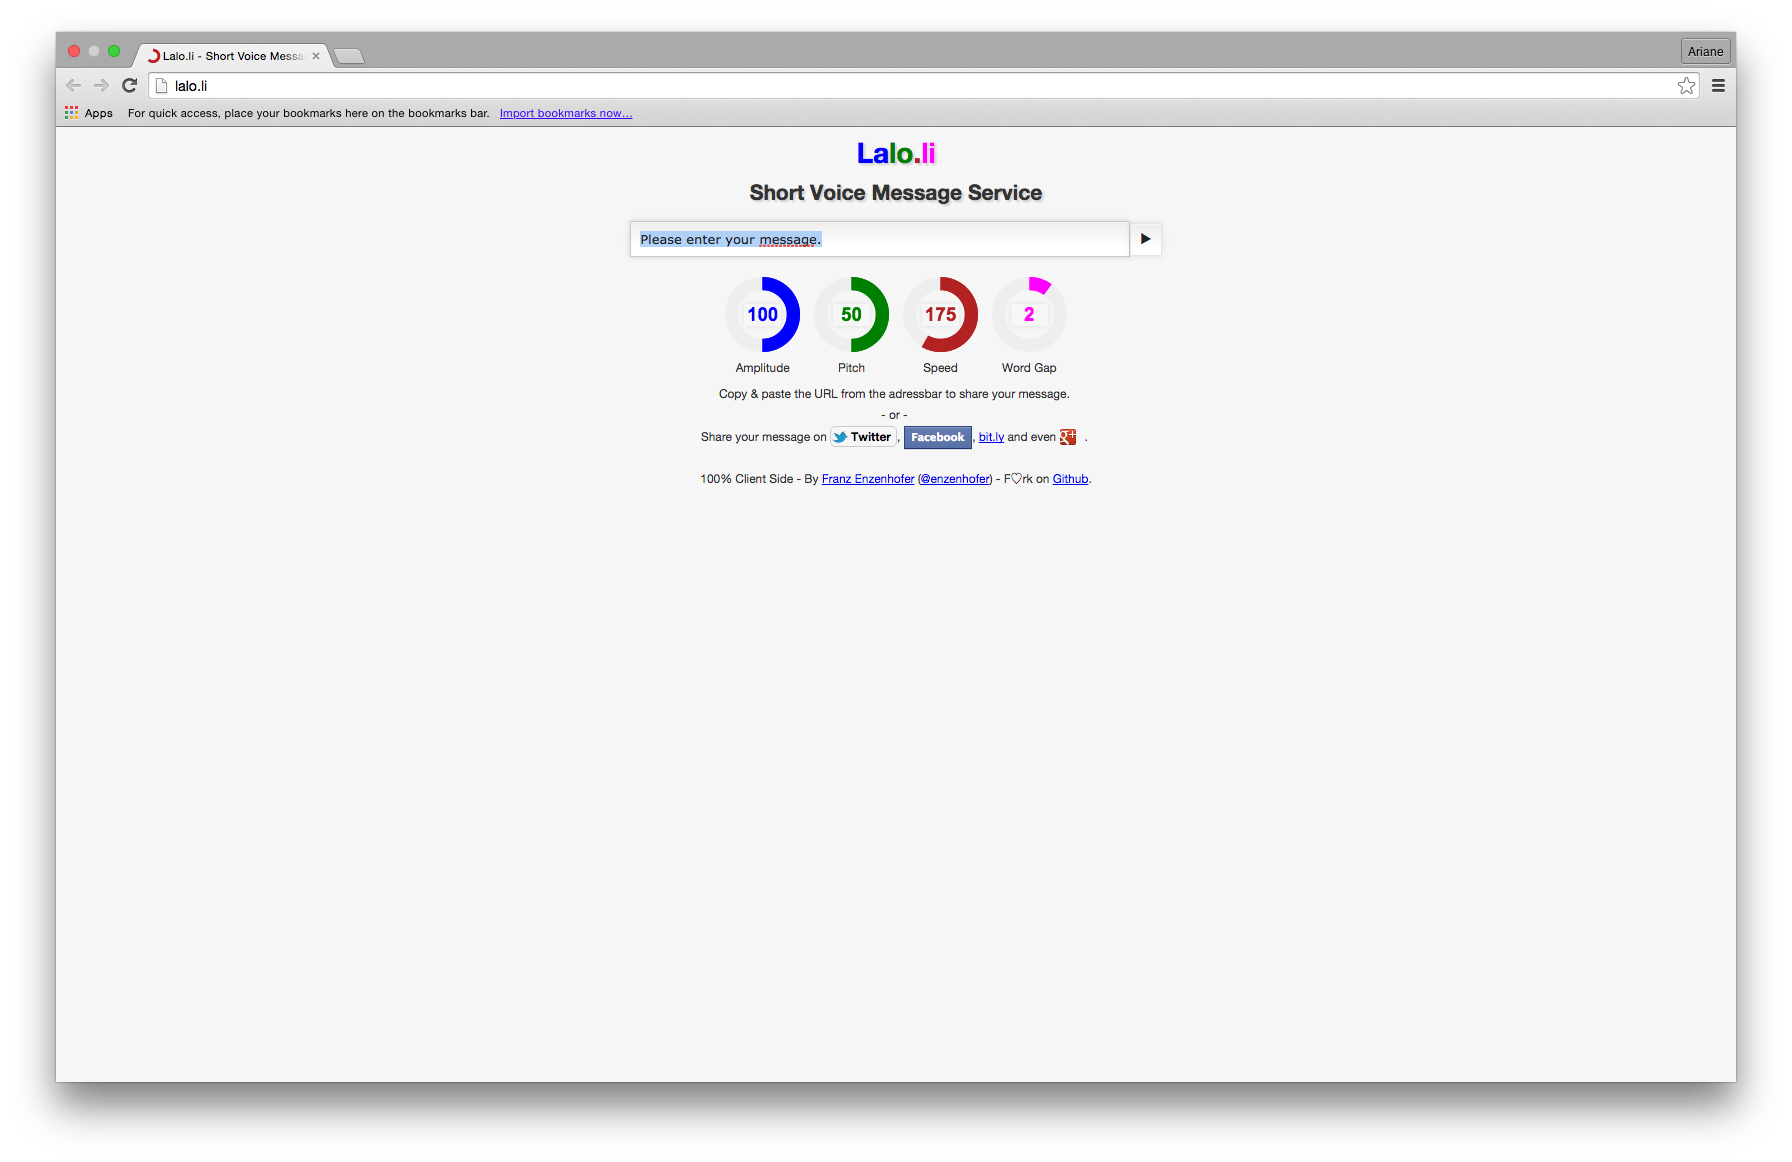
\includegraphics[width=1\linewidth]{pictures/cap2/laloli}
    
    \legend{Fonte: Screenshot da autora, dia 15 de março de 2016}
\end{figure}

O ``Spectrogram and Oscillator''\footnote{Disponível em: <http://smus.com/spectrogram-and-oscillator/>} (Figura \ref{spectrogramosc}) desenha um gráfico do espectro das frequências do som em tempo real a partir da entrada do microfone ou de um oscilador por clique. Esse experimento foi bastante interssante pois mostrou a executabilidade da análise por FFT em tempo real a partir do navegador. O sistema de síntese embutido, no entanto é bastante limitado, resumindo-se apenas a um oscilador simples.   



\begin{figure}
    \caption{\label{spectrogramosc}Interface do Spectrogram and Oscillator.}
    
        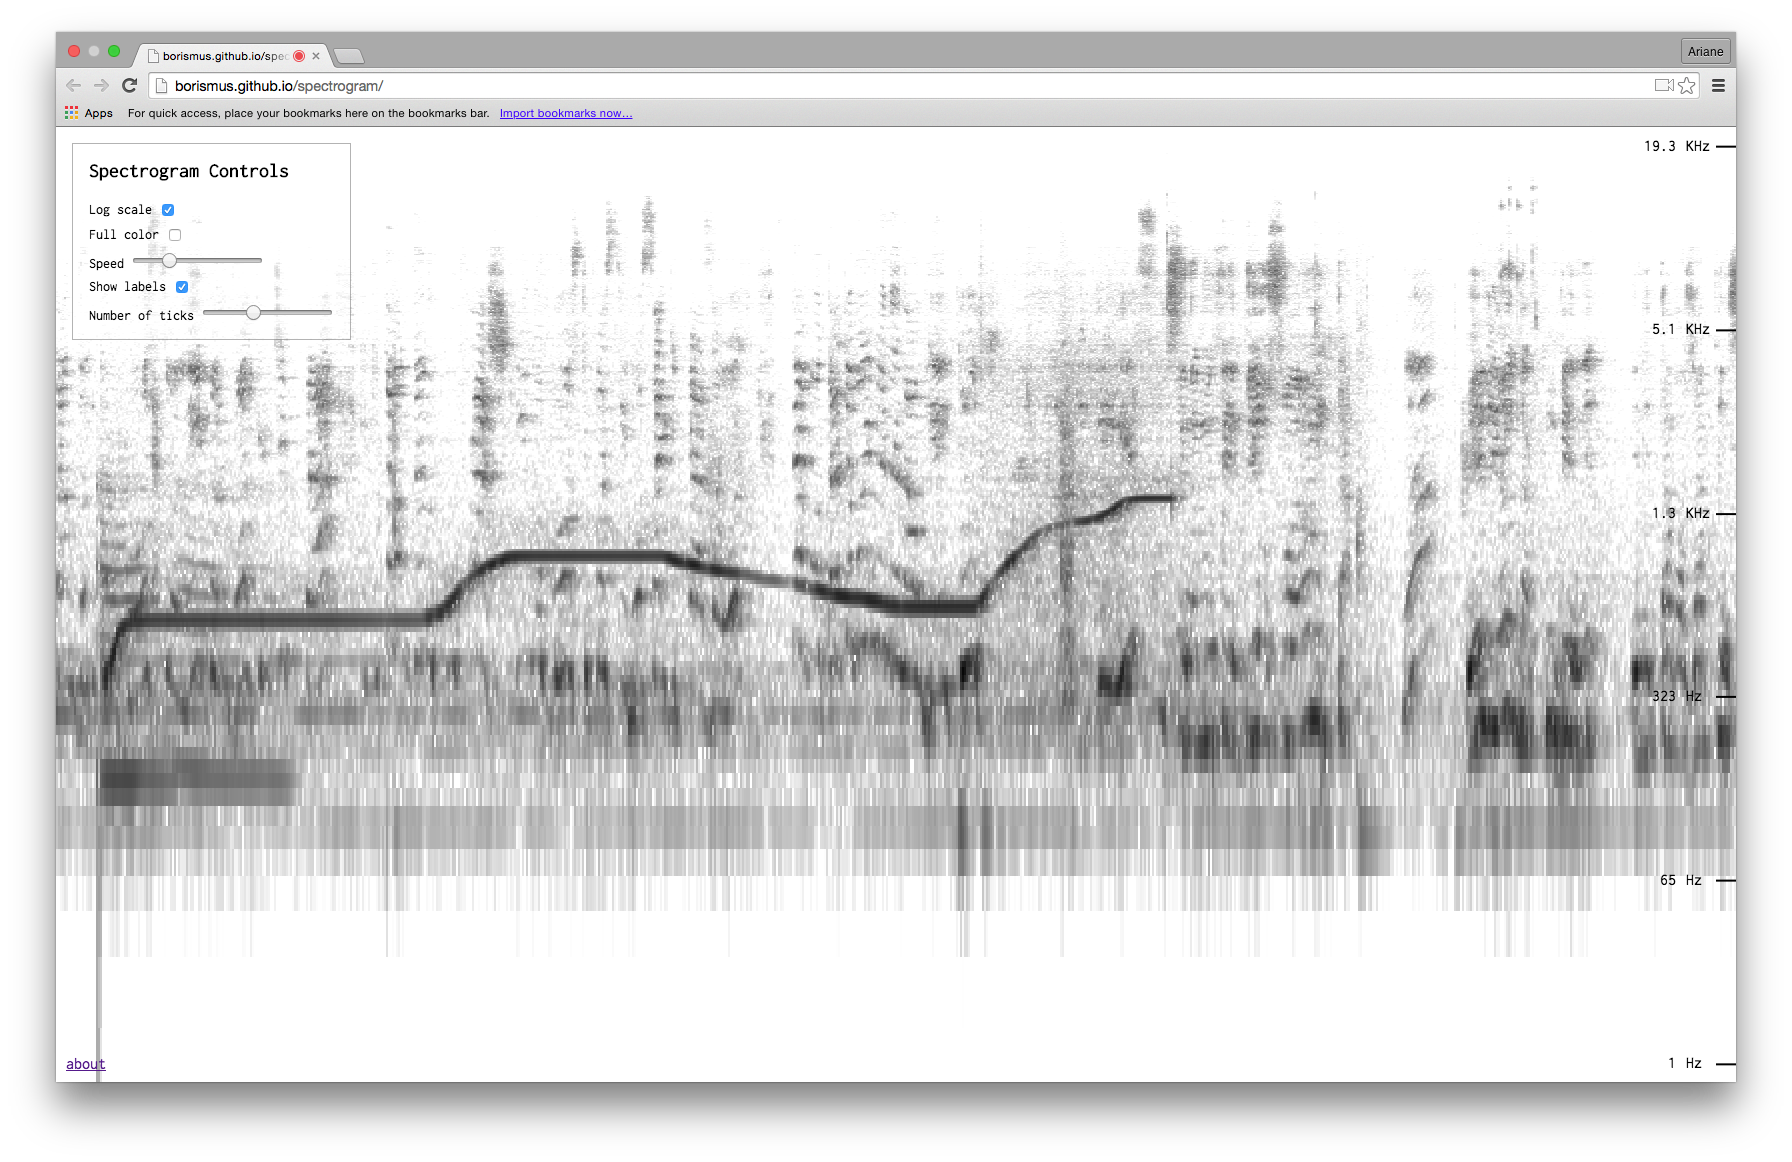
\includegraphics[width=1\linewidth]{pictures/cap2/spectrogramandoscilator}
    
    \legend{Fonte: Screenshot da autora, dia 15 de março de 2016}
\end{figure}

Patatap\footnote{Disponível em: \url{http://patatap.com}} é uma espécie de bateria eletrônica audiovisual (Figura \ref{patatap}), que usa o teclado como input. O sistema apresenta uma co-relação entre som e gráficos gerados em SVG. A quantidade de sons, no entanto, é limitada à quantidade de teclas do teclado. Os sons são fixos, e não é possível alterá-los.

\begin{figure}
    \caption{\label{patatap}Interface do Patatap.}
    
        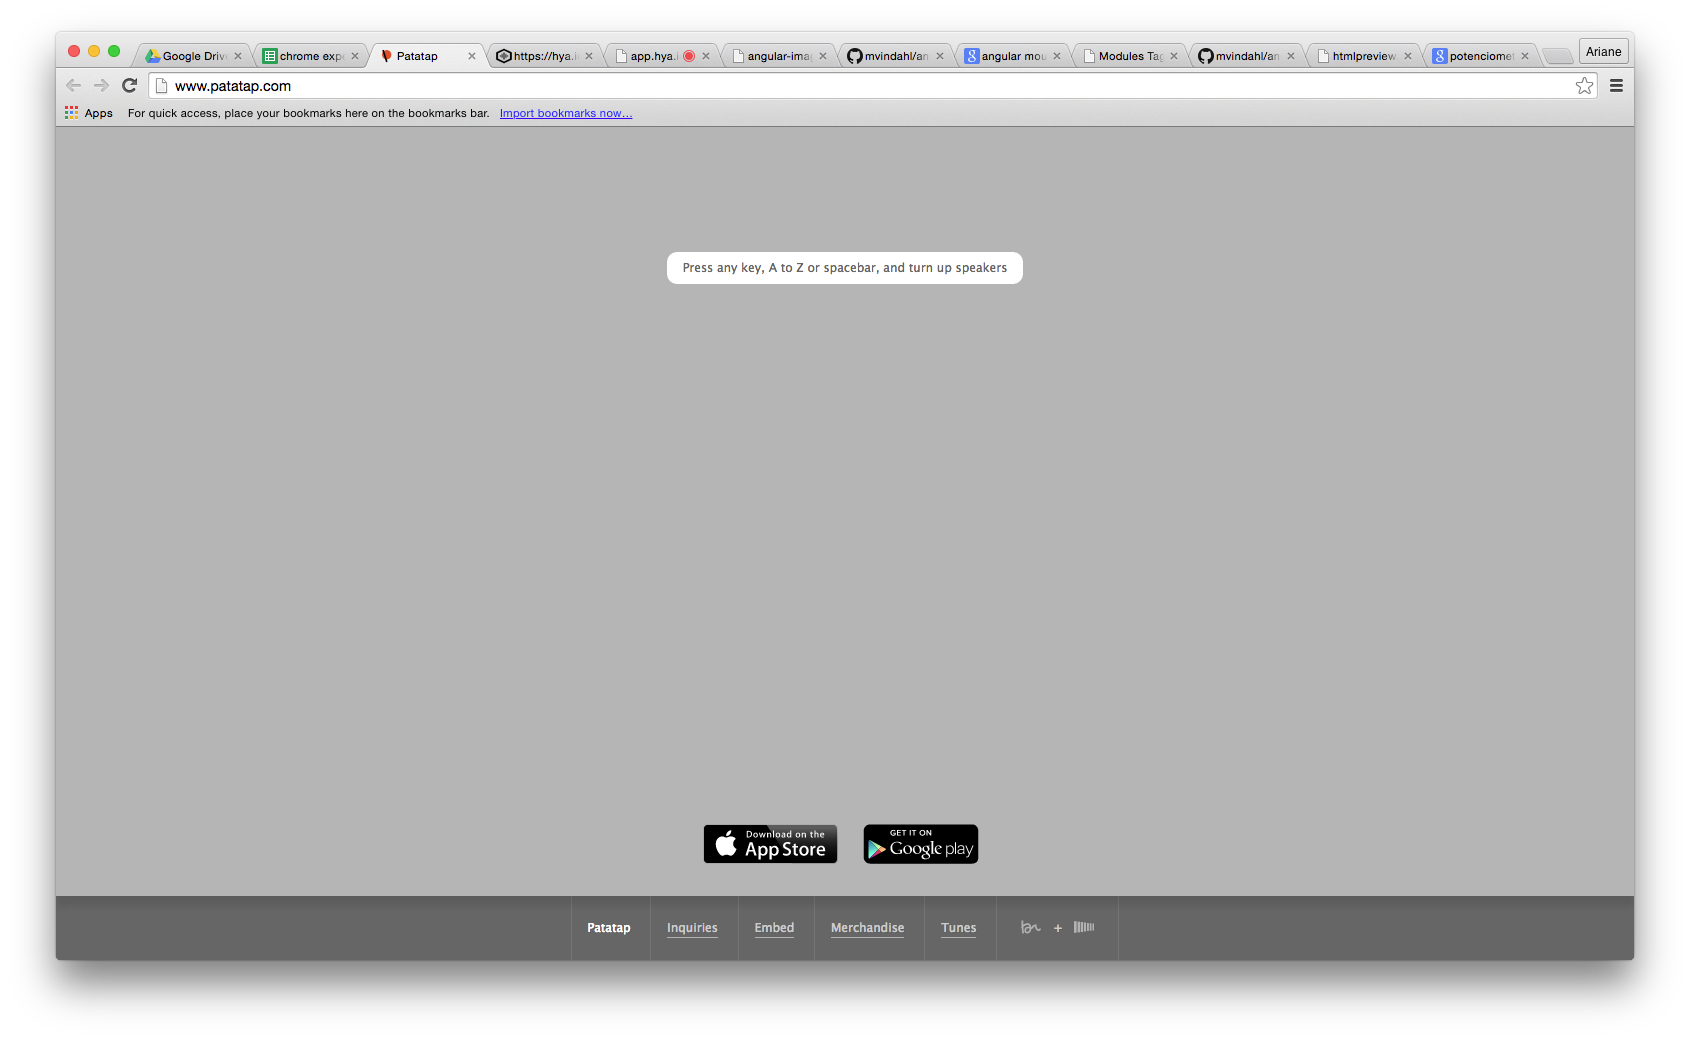
\includegraphics[width=1\linewidth]{pictures/cap2/patatap}
    
    \legend{Fonte: Screenshot da autora, dia 15 de março de 2016}
\end{figure}

Especialmente interessantes para o contexto dessa pesquisa são alguns experimentos multiusuário como o ``Plink'' (Figura \ref{plink}), onde cada pessoa que entra no site controlava um ``instrumento'' que se podia tocar com o mouse a partir de faixas verticais que representavam notas diferentes. O experimento, que não está mais no ar, tinha uma grade de tempo fixa, e os usuários que acessavam o site podiam tocar em conjunto a partir de uma lista de opções de timbres diferentes. Os instrumentos eram fixos e as notas também, e não havia possibilidade de trocar a velocidade nem alterar os timbres deles. 

\begin{figure}
    \caption{\label{plink}Interface do Plink.}
    
        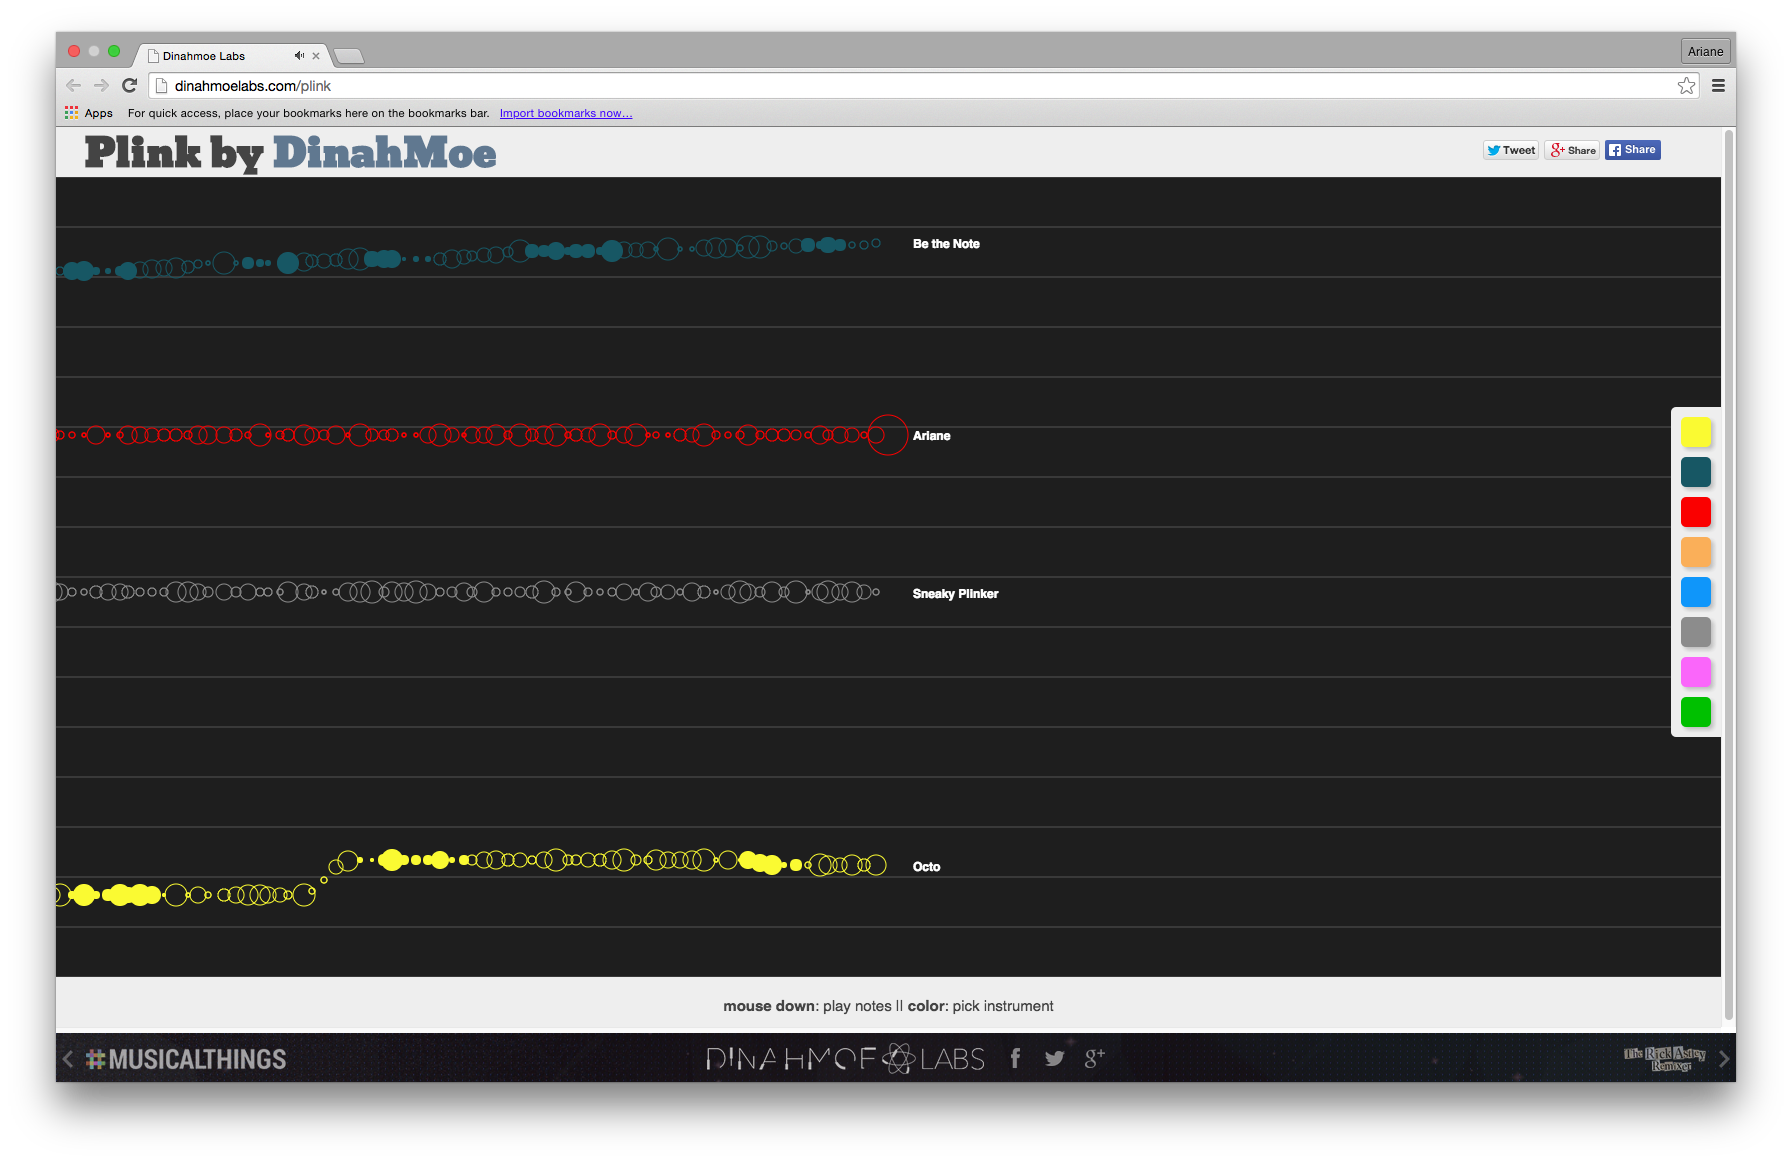
\includegraphics[width=1\linewidth]{pictures/cap2/plink}
    
    \legend{Fonte: Screenshot da autora, dia 15 de março de 2016}
\end{figure}

O ``Multiplayer Piano''\footnote{Disponível em: http://www.multiplayerpiano.com/} (Figura \ref{multiplayer}), é um piano \emph{online} aberto, onde os usuários do site se encontram virtualmente e podem tocar em conjunto. Cada usuário \emph{online} é representado por um cursor que fica circulando pela página. A interface possui um \emph{chat}, onde os usuários conversam em tempo real. Também é possível conectar o site com controladores MIDI, e é possível criar salas virtuais privadas para tocar em grupos menores. Como experiência musical, é bastante interessante, pois é um piano caótico, onde muitos tocam ao mesmo tempo. Como recuso para prática musical, no entanto é limitado, porque se limita aos sons de piano de poucas oitavas. A interface também é bastante tradicional, imitando um teclado na tela.


\begin{figure}
    \caption{\label{multiplayer}Interface do Multiplayer Piano.}
   
        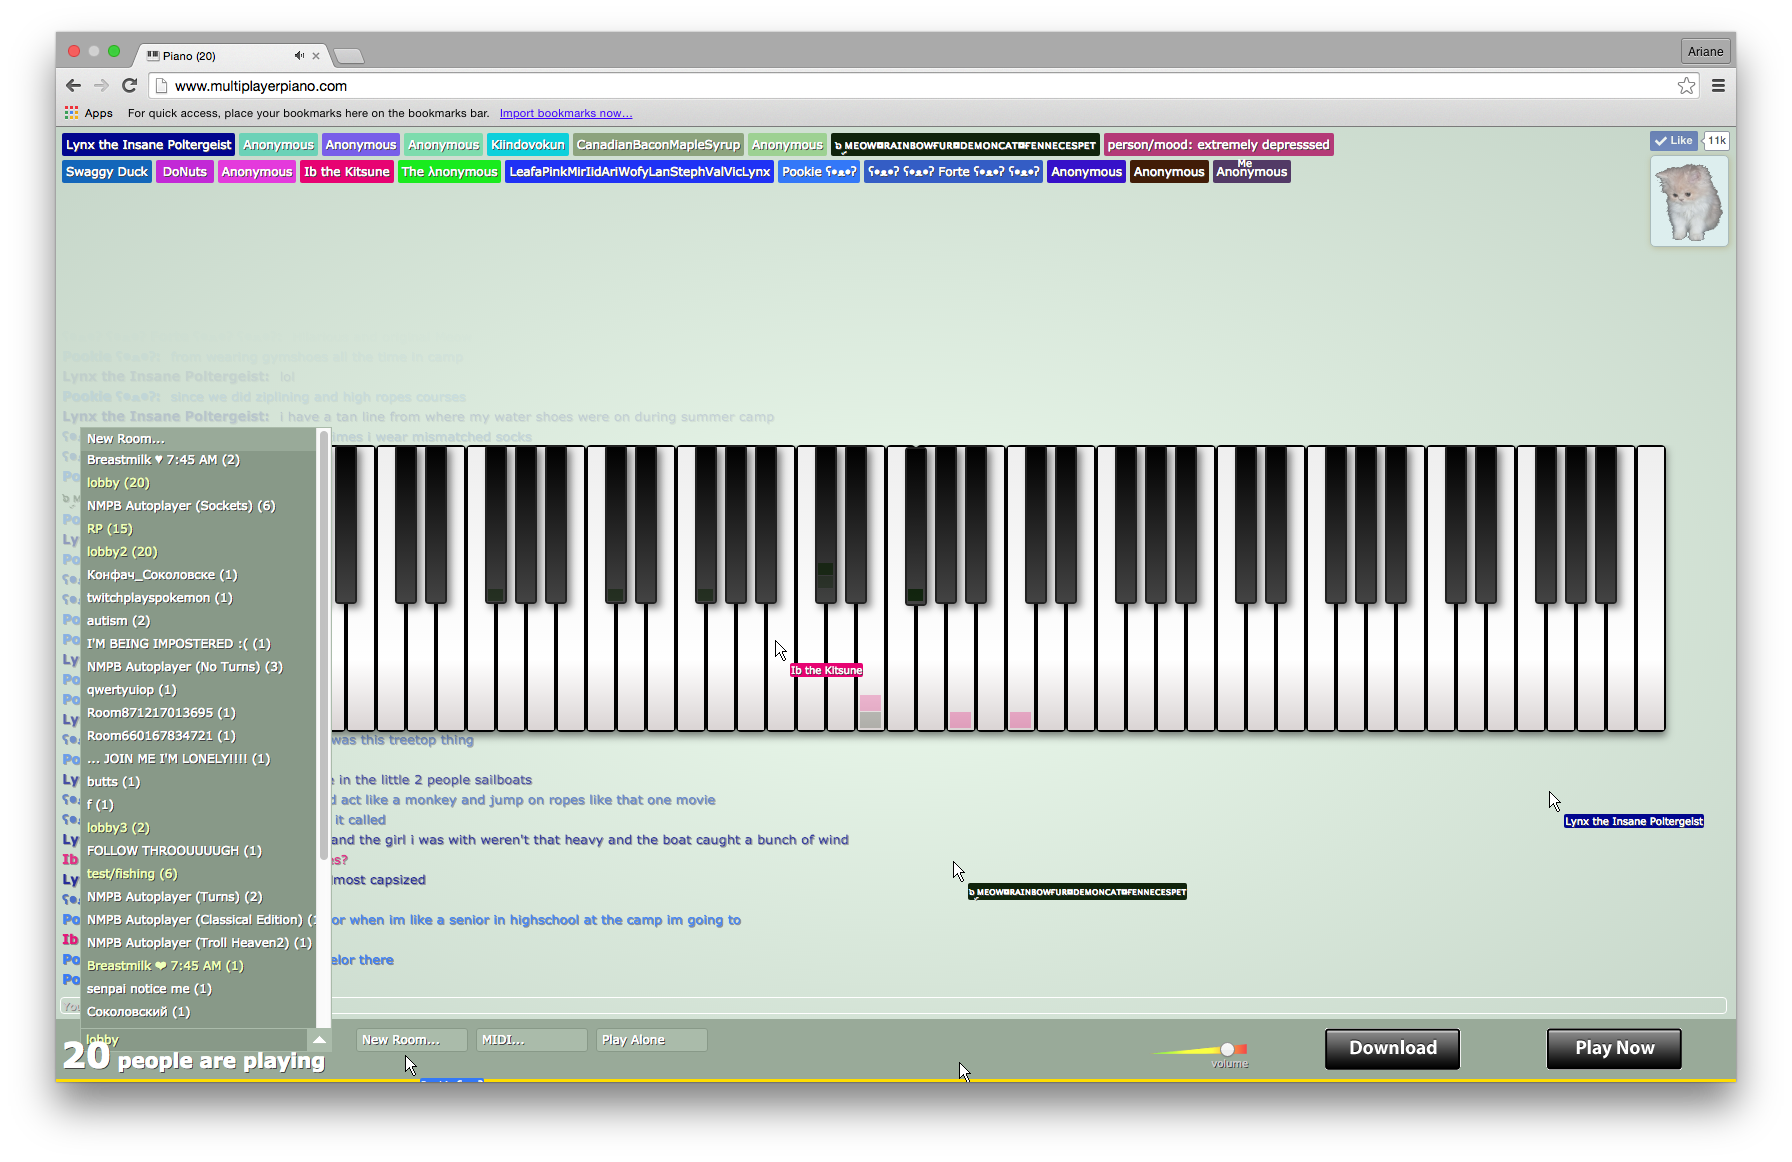
\includegraphics[width=1\linewidth]{pictures/cap2/multiplayerpiano}
   
    \legend{Fonte: Screenshot da autora, dia 15 de março de 2016}
\end{figure}


No Brasil, o projeto música móvel \footnote{\cite{Rohde2014}}, reuniu pesquisadores como Bruno Rohe, Glerm Soares e Cristiano Figueiró para produzir aplicativos de musicais para telas multique em sistema Android e software livre (Figura \ref{mmovel}). Eles usaram como base uma biblioteca que permite criar aplicativos baseados em PureData (libPD). Entre eles, o ``Looper'' \footnote{Vídeo demontrativo disponível em: https://www.youtube.com/watch?v=aTOdMNtC-sA}, que permite gravar loops em diversos canais e aplicar filtros e efeitos no domínio do tempo das frequências; B\/I\/T\/S\/L\/C (beatslicer), que ``construir
recombinações de sequenciamento de fatias de áudio''; o Photosíntese, que trabalha com síntese sonora a partir das informações de cor da imagem da câmera do celular.

\begin{figure}
    \caption{\label{mmovel}À esquerda, interface do programa looper, e à diretita do B\/I\/T\/S\/L\/C, alguns dos aplicativos desenvolvidos pelo projeto Música móvel.}
    
        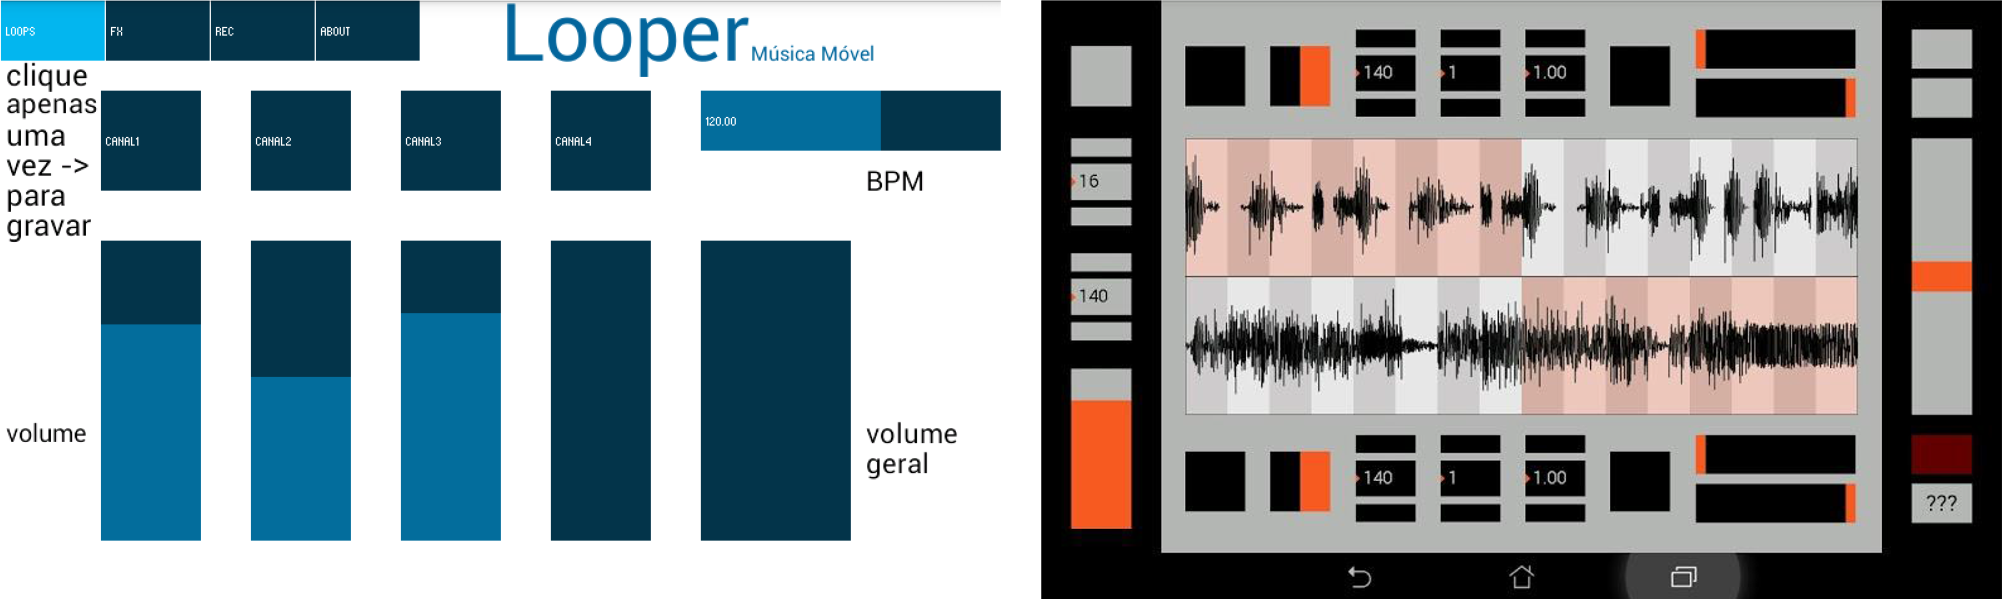
\includegraphics[width=1\linewidth]{pictures/cap2/musicamovel}
    
    \legend{Fonte: \cite{Rohde2014}}
\end{figure}

Em 2016, com a profusão de trabalhos relacionados a tecnologias web e áudio, foi organizada a primerira WebAudioConference, que foi sediada no IRCAM. Entre os tópicos da conferência, estavam: experiências inovadoras em aplicações web para áudio e música; integração multimídia; visualização de áudio nos navegadores; processamento de áudio nos navegadores; hardware e interfaces tangíveis e uso da web audio api e outros temas relacionados à aplicação de tecnologias web para áudio e música\footnote{\url{https://wac.ircam.fr/}}. Nas conferências, que aconteceram anualmente desde 2016, foram apresentados uma série de trabalhos explorando essas tecnologias para produção musical, como emuladores de DAW \footnote{\cite{Jillings2017}} ou sequenciadores \footnote{\cite{Feenstra2016}}. Com os ecperimentos que descrevemos nas próximas seções, tivemos a oportunidade de participar das dúas últimas conferências em Londres (2017) e em Berlim (2018), apresentando a versão em Web Audio do Projeto Banda Aberta\footnote{\cite{Stolfi2017b}} e o Playsound.space\footnote{\cite{Stolfi2018b}}.




%Innovative audio and music based web applications (with social and user experience aspects)
%Client-side audio processing (real-time or non real-time)
%Audio data and metadata formats and network delivery
%Server-side audio processing and client access
%Client-side audio engine and rendering
%Frameworks for audio manipulation
%Web Audio API design and implementation
%Client-side audio visualization
%Multimedia integration
%Web standards and use of standards within audio based web projects 
%Hardware, tangible interface and use of Web Audio API

%\textbf{(ii) Instrumentos musicais online.} Nos últimos anos, principalmente depois do lançamento da Web Audio API, muitas pesquisas têm sido conduzidas no desenvolvimento de plataformas para tocar música na rede. Uma parte delas são baseadas em tipos existentes de instrumentos musicais digitais, 
%\todo{incluir mais referencias aqui}


Essa diversidade de trabalhos demonstra o potencial das tecnologias web para o desenvolvimento de novas interfaces para produção musical, no entanto, a maioria dos instrumentos desenvolvidos até então ou exigiam um conhecimento prévio de técnicas musicais, ou são muitos simples e restritas em termos de expressividade musical\footnote{\cite{Dobrian2006}}, aproximando-se mais da idéia de um jogo musical do que de um instrumento propriamente dito. Apesar de mostraram que existe uma imensa potencialidade latente em explorar essas novas tecnologias, permitindo processos complexos de síntese de áudio e sampleamento, esses experimentos ainda eram relativamente precários em termos de potencialidades de produção musical, se compararmos às ferramentas disponíveis para produção musical em software, como os chamados digital audio workstations (DAW) ou os \emph{patchers}.


